\section{Integration von Erklärungen anhand des Modells}

Um eine praxisnahe Möglichkeit zu schaffen, wurde für die Anwendung des Leitfadens eine Kooperation mit der Firma \textit{Graphmasters GmbH} eingegangen. \textit{Graphmasters} ist ein in Hannover ansässiges Software-Unternehmen, welches vorwiegend Navigationssoftware entwickelt sowie Vekehrslenkungsmöglichkeiten und Tourenplanung für verschiedene Stakeholder (z.~B. Logistikunternehmen und Verkehrsmanagementzentralen) anbietet. 

Kernprodukt des Unternehmens ist eine Routing-Engine für den Straßenverkehr, welche auf Schwarmintelligenz basiert und damit alle Nutzer des Systems durch eine Cloud vernetzt. Der Algorithmus ermöglicht es, jedem Fahrzeug eine individuelle Route zuzuordnen und gibt damit jedem Teilnehmer im Schwarm die bestmögliche Route zu seinem Ziel. Diese Art von Routingalgorithmen wird \glqq Kollaboratives Routing\grqq{} genannt. Aufgrund eines Reservierungssystems erhalten Fahrzeuge mit gleichen oder ähnlichen Zielen verschiedenen Routen. Dies führt dazu, dass die vorhandene Infrastruktur besser genutzt wird.

Der große Unterschied zu herkömmlichen Navigationssystemen (\glqq Egoistisches Routing\grqq{}) ist, dass der von \textit{Graphmasters} entwickelte Algorithmus das Entstehen von Staus durch die Verteilung der Autos auf verschiedene Strecken im Vorhinein verhindert. Bekannte Navigationslösungen reagieren nur auf eine bereits vorhandene Überfüllung von Straßen. Bei Erkennung einer Überfüllung würden jedoch alle Fahrzeuge mit dem Navigationssystem auf dieselbe Alternativroute gelenkt und der Stau so nur verschoben werden. Die NUNAV genannte Technologie schafft es folglich durch Verteilungen, die Fahrzeit für alle Fahrzeuge zu verringern.

\subsection{NUNAV Navigation}

Der NUNAV-Routingalgorithmus ist bei Graphmasters in verschiedene Produkte integriert. Eines dieser ist \textit{NUNAV Navigation}. Dies ist eine frei verfügbare Navigationssoftware für Smartphones, deren Zielgruppe Endanwender sind, welche eine geführte Navigation nutzen wollen (mehr siehe \autoref{sec:06_model_evaluation:personas}). Mithilfe dieser können sich Privatanwender wie von bekannten Navigationslösungen gewohnt, zu beliebigen Zielen navigieren lassen. Darüber hinaus haben Nutzer die Möglichkeit direkt nach Veranstaltungen und von NUNAV verwalteten Orten zu suchen. Dabei können Veranstalter NUNAV als individuelles Parkleitsystem einsetzen. Navigieren Nutzer mit \textit{NUNAV Navigation} zu einem verwalteten Suchergebnis, werden sie auf einen freien Parkplatz geführt. Dabei kann auch zwischen verschiedenen Rollen unterschieden werden. So können Aussteller von Messen zum Beispiel direkt zum richtigen Eingang navigiert werden, statt auf einen Besucherparkplatz.

Für diese Arbeit dient die bestehende App \textit{NUNAV Navigation} als Grundlage für die Integration von Erklärungen und ist somit das \textit{System}, für das die Erklärbarkeit im Kontext der Anwendung des vorgestellten Leitfadens verbessert werden soll.

\subsubsection{Technischer Überblick}

Im Allgemeinen setzt die Graphmasters GmbH auf eine \textit{Micro-Service}-Infrastruktur. Das heißt, die einzelnen Teilsysteme der NUNAV-Technologie sind stark gekapselt und werden unabhängig voneinander bei mehreren Cloud-Infrastruktur-Anbietern betrieben. So ist nicht nur eine unabhängige Entwicklung möglich, sondern auch die Skalierung einzelner Systeme ist einfach und kostengünstig umsetzbar. Clients für die Services sind entweder Mobile Anwendungen für Smartphones oder Webanwendungen.

\begin{figure}[htb!]
    \centering
    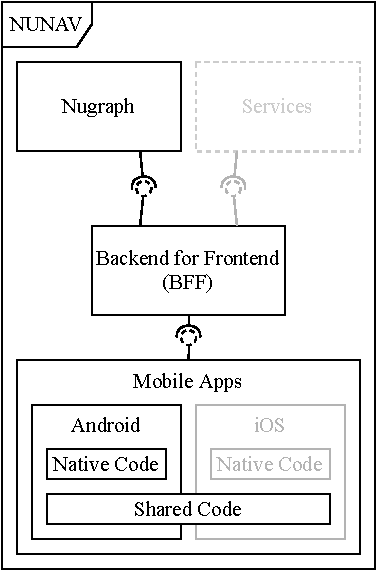
\includegraphics[width=\textwidth]{contents/06_model_evaluation/01_integration/res/nunav_architecture.pdf}
    \caption{Ausschnitt aus der NUNAV Software Architektur (UML-Komponenten-Diagramm)}
    \label{fig:nunav_software_architecture}
\end{figure}

\autoref{fig:nunav_software_architecture} stellt abstrakt alle für diese Arbeit relevanten Services der Infrastruktur dar. Wichtig ist dabei zum einen der Routingalgorithmus an sich (\textit{Nugraph}), welcher die Daten für die Navigation bereitstellt. Zum anderen ist die Mobile Anwendung von \textit{NUNAV Navigation} relevant, da dort Erklärungen integriert werden sollen. Außerdem gibt es für jede Client-Anwendung einen sogenannten BFF (\textit{Backend for Frontend}). Für diese Arbeit ist der \textit{Mobile BFF} relelvant. Dieser stellt die einzige Kommunikationsschnittstelle der Clients mit allen anderen Services der Infrastruktur dar. In der Regel wird die Kommunikation zwischen den Services bzw. Clients und dem BFF über REST
\footnote{\textit{Representational State Transfer} ist ein Paradigma zum Austausch von Daten über das HTTP-Protokoll.}
-Schnittstellen mit JSON
\footnote{\textit{JavaScript Object Notation} ist ein Datenformat, welches vor allem für Maschine-zu-Maschine-Kommunikation eingesetzt wird und Programmiersprachen unabhängig ist.}
als Übertragungsformat abgewickelt. 

\paragraph{Nugraph} \textit{Nugraph} ist der Gesamtbegriff in der Architektur für die Services, welche zum Routingalgorithmus gehören. Dieser berechnet auf der Basis eines prädiktiven Verkehrsmodells die individuell schnellste Route zwischen zwei Punkten. Dabei wird anhand von ca. 1,5 Millionen Verkehrsmessungen
 (z.B. \textit{Floating Car Data}\footnote{\textit{Floating Car Data} (FCD) sind mit Zeitstempeln versehene Geolokalisierungs- und Geschwindigkeitsdaten, die direkt von fahrenden Fahrzeugen erfasst werden})
 in der Minute der Verkehr auf der Route zum Zeitpunkt, zu dem Nutzer durch den Verkehr an einer Stelle beeinflusst werden, mithilfe von Künstlicher Intelligenz vorausgesagt. Alle Daten die zur Navigation (z.b. Verlauf und Geschwindigkeit auf der Route) benötigt werden kommen von diesem Teilsystem.

\paragraph{Backend for Frontend} Der in \autoref{fig:nunav_software_architecture} gezeigte \textit{Mobile-BFF} ist zum einen für die korrekte Weiterleitung von Anfragen an den richtigen Service zuständig. Darüber hinaus bereitet dieser auch Daten anderer Services für die Mobilen Apps auf oder konvertiert die verschiedenen Formate. Dabei werden zum Teil Daten mehrerer Services gebündelt oder neue Daten berechnet. 

\paragraph{Mobile Apps} Die mobilen Anwendungen für Smartphones bereiten zum einen die Daten der \textit{Micro-Services} für die Nutzer auf und zeigen sie diesen an. Zum anderen verarbeiten diese lokal die vom BFF bereitgestellte Routen und berechnen die Position auf dieser, zum Geben von Abbiege-Kommandos und Anzeigen des Routenverlaufs. Die \textit{Mobile Apps} werden für Android und iOS parallel in den jeweiligen vom Hersteller bereitgestellten Frameworks nativ entwickelt. Außerdem gibt es eine geteilte Code-Basis, welche Kotlin-Native\footnote{\textit{Kotlin-Native} ist eine Technologie zur Kompilierung von Kotlin-Code in Binärdaten für verschiedene Platformen und Prozessorarchitekturen.} als Technologie nutzt.

\bigskip

Die drei vorgestellten Systemteile sind jene, welche entweder Daten für Erklärungen liefern können, oder für die Auslieferung von Erklärungen an die \textit{End User} fungieren. Im Rahmen dieser Arbeit wurden dabei sowohl auf dem BFF, als auch in der Mobilanwendung für Android Änderungen vorgenommen. Außerdem wurden durch Änderungen von der Graphmasters GmbH in \textit{Nugraph} und einem weiteren Service vorgenommen, um benötigte Daten für die entwickleten Erklärungen zur Verfügung zu stellen.

\subsection{Ermittlung des Erklärungsbedarfs}
\label{sec:explanation_demand_generation}

Die Anwendung des Leitfadens zur Integration von Erklärungen ist in mehrere Teile gegliedert. In einem ersten Schritt wurden die existierenden Verständnisprobleme in NUNAV analysiert. Diese wurden aus verschiedenen Datenquellen der \textit{Graphmasters GmbH} zusammengefasst. Dazu zählen unter anderem mehrere Support-Kanäle.

Um diese Analyse anzureichern, wurde darauf aufbauend ein Workshop mit mehreren Mitarbeitern der \textit{Graphmasters GmbH} durchgeführt. Ergebnis diesen Workshops waren dann eine Aufstellung der Probleme, Ziele und Rohanforderungen für Erklärungen und Ideen zur Umsetzung. Auf Basis dieser Ergebnisse wurden dann im Rahmen dieser Arbeit die Anforderungen konkretisiert und in Designs für Erklärungen umgesetzt. Abschließend ist die technische Realisierung in \textit{NUNAV Navigation} erfolgt.

\subsubsection{User-Feedback-Analyse}

Für die initiale Analyse, welche Verständnisprobleme in \textit{NUNAV Navigation} bestehen, wurde zunächst manuell das Feedback, welches im Google Play Store und Apple App Store von Nutzern in Form von App-Reviews gegeben wurde, analysiert (ab Oktober 2020). Daraus sind Themengebiete abgeleitet worden, und die Anzahl der Reviews, die ein Themengebiet ansprechen, wurden gezählt. Aus insgesamt 304 Reviews konnten 46 identifiziert werden, aus denen klare Themen abgeleitet werden können. 33 dieser Review thematisieren Verständnisprobleme. Die Themen, die häufig vorkamen und für Erklärbarkeit relevant sind, sind in \autoref{sec:appendix_literature_research} aufgelistet. Dabei wurde als Hauptproblem ein zu geringes Verständnis für den kollaborativen Routing-Algorithmus identifiziert. Allein fünf der 16 Reviews, aus denen sich dies ableiten lässt, bemängeln, dass NUNAV keine Alternativrouten vorschlägt. Dies weist darauf hin, dass nicht klar ist, dass das System des Verteilens der Nutzer auf die vorhandene Verkehrsinfrastruktur nur möglich ist, wenn die Nutzer den vorgeschlagenen Routen folgen und keine Alternativen nehmen.

Außerdem gibt es Hilfe-Artikel, die über einen \textit{Hilfe-Center} der \textit{Graphmasters}-Webseite erreichbar sind\footnote{\url{https://support.graphmasters.net/}, besucht: 01.10.21}. Dabei wurden die Klickzahlen mit den Review-Anzahlen verglichen, welche vom Verhältnis her ähnlich der Anzahlen an Reviews ist.

Aus den Reviews und Hilfe-Center-Artikeln wurden dann erste Themen beziehungsweise Nutzerfragen abgeleitet und mit dem Team \glqq Solution Experts\grqq{} von \textit{Graphmasters} diskutiert. Das Team ist für die Betreuung von Kunden und die Bearbeitung von Feedback zuständig. Die Ergebnisse sind in \autoref{tab:06_model_evaluation_explicit_questions} zu sehen.

\begin{table}[htb!]
    \begin{tabular}{p{.3\textwidth}p{.66\textwidth}}
        \hline
        Thema         & Fragen \\
        \toprule
        Kollaboratives Routing  & Was ist / wie funktioniert kollaboratives Routing? \\
        &  Warum brauche ich eine ständige Internetverbindung? \\
        &  Wieso werden in NUNAV keine Standardrouten angezeigt?\\
        \tablerowspacing
        Navigation              & Warum wird diese Route / der Umweg genommen? \\
        & Warum sind die Routen bei NUNAV länger? \\
        & Warum ist die Position ungenau? \\
        \tablerowspacing
        Vertrauen in das System & Woher kommen die Verkehrs-/ Sperrungsdaten? \\
        & Was passiert mit meinen Daten? \\
        & Wofür benötige ich Ortungsdienste beim App-Start? \\
        & Kann die Güte der Route nicht bewerten? \\
        \tablerowspacing
        Funktionen   & Was zeigt die Rainbow-Route an? \\
        & Wie kann ich eine Sperrung melden? \\
        & Wie kann ich mein Ziel in NUNAV eingeben? \\
        & Wie kann ich Favoriten anlegen? \\
        \toprule
    \end{tabular}
\caption{Anzahl der Reviews im Google Play Store und Apple App Store mit mehrfach vorkommenden Themen}
\label{tab:06_model_evaluation_explicit_questions}
\end{table}

\bigskip

Auf Basis dieser ersten Ergebnisse wurde im Anschluss ein Workshop mit mehreren \textit{Graphmasters}-Mitarbeitern durchgeführt.

\subsubsection{Workshop zur Integration von Erklärungen}

Zum Festlegen der Ziele und Anforderungen an die Erklärungen sowie zum Sammeln erster Umsetzungsideen, wurde ein interdisziplinärer Workshop mit Frontend-Entwicklern, \glqq Solution Experts\grqq{} und einem Produktmanager bei \textit{Graphmasters} durchgeführt. Außerdem sollten Metriken gefunden werden, welche zur Überprüfung der Ziele verwendet werden können. Durch die direkte Anwendung des entwickelten Leitfadens im Workshop konnten außerdem Beobachtungen darüber, wie dieser eingesetzt wird, gesammelt werden. Dies war allerdings nicht Kern des Workshops. 

Nach der initialen Vorstellung von Erklärbarkeit, dem Leitfaden für die Integration von Erklärungen sowie den Ergebnissen aus der User-Feedback-Analyse hat sich der Workshop an dem Aufbau des Modells für Erklärungen orientiert. Folglich wurden zuerst Informationen zu möglichen Nutzern (\textit{Context}), dann Ziele (\textit{Objectives}) und deren Umsetzungsmöglichkeiten (\textit{Characteristics}) und schließlich die Evaluationsmöglichkeiten besprochen (\textit{Evaluation}). Auch wenn der Workshop so geplant war, dass die einzelnen Aspekte nacheinander abgearbeitet werden, hat sich ergeben, dass die Ziele und deren Umsetzung gleichzeitig behandelt wurden. Grund dafür war, dass beim Aufstellen der Ziele und Rohanforderungen bereits die Umsetzbarkeit im Rahmen dieser Arbeit diskutiert wurde. Einige Fragen der Machbarkeit sind allerdings ungeklärt geblieben, da hierfür Wissen von den Entwicklern des Routing-Algorithmus benötigt wurde. Explizit ging es um die Frage, welche Daten für bestimmte Erklärungen überhaupt zur Verfügung gestellt werden können. Ein detailliertes Ergebnisprotokoll des Workshops ist in \autoref{sec:appendix_workshop_protocol} zu finden.

\newpage

Aus den Ergebnissen des Workshops wurden dann iterativ und in Rücksprache mit verschiedenen Teilnehmern des Workshops Personas, die konkreten Anforderungen sowie die finalen Erklärungen, die in \textit{NUNAV Navigation} integriert werden sollten, entwickelt.

\subsection{Personas von NUNAV-Nutzern}
\label{sec:06_model_evaluation:personas}

Um die Interpreation der Rohanforderungen aus dem durchgeführten Workshop besser interpretieren zu können, wurden Personas für typische NUNAV-Nutzergruppen abgeleitet. Graphmasters hat zwar kein genaues Bild, darüber welche Nutzertypen \textit{NUNAV Navigation} nutzen, aus einzelnen Nutzer-Gesprächen aus der Vergangenheit haben sich allerdings zwei Gruppen herauskristalisiert, die klar benennbar sind.

\begin{wrapfigure}{o}{0.33\textwidth}
    \vspace{-\intextsep}
    \centering
    
\includegraphics[width=0.3\textwidth]{contents/06_model_evaluation/01_integration/res/persona_picture_michael.png}
    \caption{Michael -\\Lizensiert bei Shutterstock Nr. 602783837}
\end{wrapfigure}

\paragraph{Vielfahrer} Michael, 34 Jahre alt, arbeitet als Unternehmensberater in einem großen Beratungsunternehmen. Er hat Betriebswirtschaftleere studiert und ist seit dem Studium in der Firma.

Er wohnt mit seiner Frau und einer Tochter in der Vorstadt und muss jeden morgen zur Hauptverkehrsszeit in die Stadt fahren, um in sein Büro zu kommen. Dadurch steht er nahezu täglich im Stau auf dem Weg zur Arbeit. Die öffentlichen Verkehrsmittel kommen für ihn nicht in Frage, da er mit ihnen mehr als doppelt so lange bräuchte. Auch zu Vortortterminen beim Kunden fährt er ungefähr einmal pro Woche. Dabei interessiert ihn vor allem, wie hoch das Verkehrsaufkommen zu dem Zeitpunkt auf der Strecke ist.

Lange Zeit hat er das in sein Auto integrierte Navigationssystem verwendet, das aber nur vereinzelt auf Staus reagiert hat und ihn jeden Tag auf der gleichen Strecke zur Arbeit geschickt hat, wenn nicht ein besonderes Ereignis wie Unfälle oder Sperrungen auf der Strecke waren.

Michael hat ein modernes Dienst-Smartphone mit Android und ist generell technik interessiert. Zwischendurch hat er die auf seinem Smartphone vorinstallierte Navigations-App verwendet, da diese immer aktuellen Verkehr anzeigen kann. Diese leitetete ihn zum Teil aus dem Stau des Berufsverkehrs raus, in dem er stand. Er hat aber meist ähnlich lange zur Arbeit gebraucht wie im Stau. Außerdem achtet Michael darauf, was mit seinen Daten passiert und da ist er sich bei dem Anbieter nicht sehr sicher, wie anonym diese verarbeitet werden.

Seit einigen Tagen verwendet er die Navigations-App \text{NUNAV Navigation}, die verspricht ihn jeden Tag auf dem schnellsten Weg zur Arbeit zu bringen. Die App schlägt ihm ab und zu seiner Meinung nach \glqq komische\grqq{} Routen vor. Anfangs hat er sich dann nicht an diese gehalten. Dann hat er die Alternativen ausprobiert. Tatsächlich war er etwas schneller als sonst auf dem Weg zur Arbeit. Er ist aber immer noch skeptisch, da er die vorgeschlagenen Routen nicht immer versteht und bei sich bei Umwegen immer noch auf seine Intuition verlässt.

\bigbreak

\begin{wrapfigure}{o}{0.33\textwidth}
    \vspace{-\intextsep}
    \centering
    
\includegraphics[width=0.3\textwidth]{contents/06_model_evaluation/01_integration/res/persona_picture_ayla.png}
    \caption{Ayla -\\Lizensiert bei Shutterstock Nr. 1433736386}
\end{wrapfigure}

\paragraph{Erstnutzer} Ayla ist 23 Jahre alt und studiert aktuell Mathematik im 7. Bachelorsemester. Sie wohnt in einem Studentenwohnheim und fährt jeden Tag mit der Bahn zur Universität. Sie kommt ursprünglich aus einem Dorf ca. 300~km entfernt besucht ihre Eltern dort mindestens dreimal im Monat am Wochenende. Dafür hat sie ein Auto, da sie mit ihrem Semesterticket nicht bis in die Heimat fahren kann.

% 2. Event-Fahrer (Erste Nutzung, kennt den kollaborativen Ansatz nicht.) Lorem ipsum dolor sit amet, consetetur sadipscing elitr, sed diam nonumy eirmod tempor invidunt ut labore et dolore magna aliquyam erat, sed diam voluptua. At vero eos et accusam et justo duo dolores et ea rebum. Stet clita kasd gubergren, no sea takimata sanctus est Lorem ipsum dolor sit amet. Lorem ipsum dolor sit amet, consetetur sadipscing elitr, sed diam nonumy eirmod tempor invidunt ut labore et dolore magna aliquyam erat, sed diam voluptua. At vero eos et accusam et justo duo dolores et ea rebum. Stet clita kasd gubergren, no sea takimata sanctus est Lorem ipsum dolor sit amet.

% Lorem ipsum dolor sit amet, consetetur sadipscing elitr, sed diam nonumy eirmod tempor invidunt ut labore et dolore magna aliquyam erat, sed diam voluptua. At vero eos et accusam et justo duo dolores et ea rebum. Stet clita kasd gubergren, no sea takimata sanctus est Lorem ipsum dolor sit amet. Lorem ipsum dolor sit amet, consetetur sadipscing elitr, sed diam nonumy eirmod tempor invidunt ut labore et dolore magna aliquyam erat, sed diam voluptua. At vero eos et accusam et justo duo dolores et ea rebum. Stet clita kasd gubergren, no sea takimata sanctus est Lo

\subsection{Anforderungen der Erklärungen}

Mithilfe der Rohanforderungen und Ziele aus dem Workshop sowie den erstellten Personas können sowohl funktionale als auch nicht-funktionale Anforderungen für Erklärungen in NUNAV entwickelt werden

\subsubsection{Nicht-Funktionale Anforderungen}

% \cite{kohl_explainability_2019} gives a good overview to the requirement analysis for Explainability as an NFR

Als Methode zum Ableiten der konkreten NFRs wurde das Aufstellen eines Qualitätsmodells gewählt \cite{schneider2012abenteuer}. Das Modell ist in \autoref{fig:nunav_explanation_quality_model} dargestellt. Bei der Erstellung wurde iterativ Rücksprache mit den verschiedenen Teilnehmern des Workshops gehalten. Als Basis für die Qualitätsziele wurden die in dem Modell für Erklärungen unter \textit{Objectives} aufgeführten Ziele verwendet. Die Endfassung der Anforderungen wurde schlussendlich vom Teamleiter des \glqq Mobile Application\grqq{}-Teams abgesegenet.

Es hat sich allerdings herausgestellt, dass das Aufstellen solch konkreter Anforderungen nicht der Arbeitsweise von Graphmasters entspricht. In den Rücksprachen wurde klar, dass die Ziele normalerweise deutlich abstrakter gehalten werden. Für eine Evaluation der Integration von Erklärungen im Rahmen dieser Arbeit werden die konkreten Anforderungen zur Prüfung allerdings benötigt.

\begin{figure}[htb!]
    \centering
    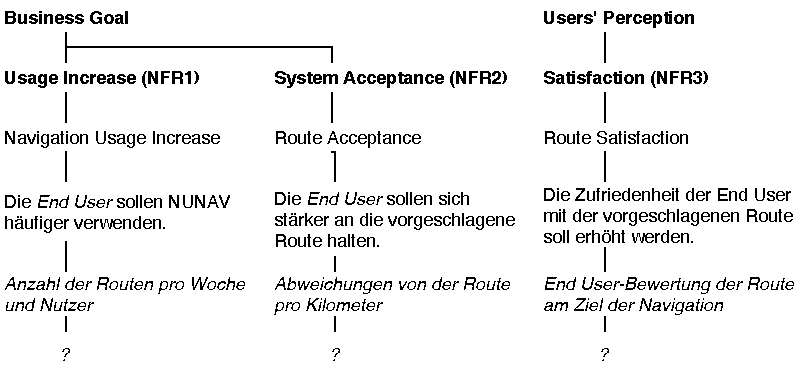
\includegraphics[width=\textwidth]{contents/06_model_evaluation/01_integration/res/quality_model.pdf}
    \caption{Qualitätsmodell für die Integration von Erklärungen in NUNAV Navigation}
    \label{fig:nunav_explanation_quality_model}
\end{figure}

In \autoref{fig:nunav_explanation_quality_model} ist zu erkennen, dass für Graphmasters im Allgemeinen die Erhöhung der Nutzung und die Akzeptanz des Systems im Vordergrund stehen. Bei der Nutzung ist für Graphmasters die interessanteste Metrik die Anzahl der aktiven Nutzer. Da sich eine Messung von Veränderungen dieser durch die Integration von Erklärungen allerdings nicht über einen kurzen Zeitraum messen lässt, wurde  als Metrik die Anzahl der Routen pro Nutzer und Woche vorgeschlagen und schließlich auch durch Graphmasters bestätigt. Für die Akzeptanz des Systems ist ein Ziel, dass sich die \textit{End User} möglichst viel an die vorgeschlagene Route halten. Als Metrik wurde hierfür die Anzahl der Abweichungen von der Route pro Kilometer verwendet.

Ein weiteres wichtiges Ziel von Graphmasters ist die Zufriedenheit der \textit{End User} mit den Routen. Hierfür bestand bereits vor dem Beginn dieser Arbeit eine Metrik. \textit{End User} können bei Erreichen des Ziels einer Navigation auf einer Skala mit ein bis fünf Sternen angeben, wie zufrieden sie insgesamt mit der Route waren. Bis dato wurde diese Metrik allerdings noch nicht systematisch ausgewertet.

Für alle Metriken fällt auf, dass in \autoref{fig:nunav_explanation_quality_model} keine Sollwerte definiert sind. Aus den Gesprächen hat sich ergeben, dass für Graphmasters erstens nicht wichtig ist, um wie viel die verschiedenen Metriken sich verbessern, solange mit der Integration von Erklärungen eine Besserung eintritt. Außerdem ist sind keine Basiswerte vorhanden, auf die man sich beziehen kann. Aus diesem Grund wurden die konkreten Anforderungen in Bezug auf signifikante Unterschiede formuliert. Die Formulierungen orientieren sich dabei an gängigen Vorlagen, enthalten allerdings nicht die in den Vorlagen geforderten Sollwerte \cite{rajnish2010quality, wiegers1999writing, alexander2002writing}:

\begin{enumerate}
    \item [NFR1] Die Anzahl der gefahrenen Routen mit \textit{NUNAV Navigation} pro Nutzer und Woche soll signifikant messbar erhöht werden.
    \item [NFR2] Die durchschnittliche Anzahl der Abweichungen der Nutzer pro Kilometer von der durch \textit{NUNAV Navigation} vorgeschlagenen Route soll signifikant messbar verkleinert werden.
    \item [NFR3] Die durchschnittliche Bewertung der Route am Ende der Navigation in \textit{NUNAV Navigation} soll signifikant messbar erhöht werden.
\end{enumerate}

\subsubsection{Funktionale Anforderungen}

In diesem konkreten Fall stand die Integration von Erklärungen als Lösungsansatz zum Erreichen der Ziele bereits fest. Daher wurden die \textit{Explanation Goals} aus dem Modell für Erklärungen ausgewählt, welche in Erklärungen umgesetzt werden sollten. Dabei steht vor allem auch die Frage im Raum, welche Aspekte genau erklärt werden müssen \cite{kohl_explainability_2019}.

Ein Ergebnis des durchgeführten Workshops war die Verständnisprobleme der Nutzer, welche durch Erklärungen gelöst werden sollen und erste Umsetzungsideen. Aus diesen beiden Punkten konnten \textit{Transparency} und \textit{Scrutability} als Ziele für die Integration von Erklärungen abgeleitet werden.
% Da die vorherigen Qualitätsanforderungen sehr Allgemein auf \textit{NUNAV Navigation} bezogen sind, ist das Ziel, dass sich alle integrierten Erklärungen positiv auf die Qualitätsziele auswirken.

Auch die Konkretisierung der funktionalen Anforderungen ist iterativ erfolgt. Eine Herausforderung dabei war vor allem, dass Graphmasters in der Regel keine konkreten Anforderungen formuliert, sondern direkt anhand von Ideen Mockups erstellt und dann iterativ mehrere Prototypen entwickelt.

Für die funktionalen Anforderungen wurde ein Zielbaum ähnlich zu Qualitätsmodellen aufgestellt, in dem die Konkretisierungsschritte zu sehen sind. \autoref{fig:nunav_explanation_functional_model} stellt diesen dar.

\begin{figure}[htb!]
    \centering
    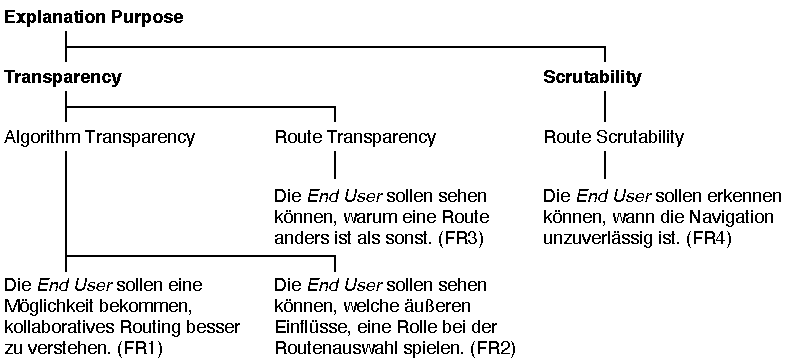
\includegraphics[]{contents/06_model_evaluation/01_integration/res/functional_model.pdf}
    \caption{Konkretisierungsschritte bei der Entwicklung der funktionalen Anforderungen an Erklärungen in \textit{NUNAV Navigation}}
    \label{fig:nunav_explanation_functional_model}
\end{figure}

Aus den Konkretisierungsschritten (siehe \autoref{fig:nunav_explanation_functional_model}) wurden schlussendlich folgende funktionalen Anforderungen abgeleitet:
% . Die in der Abbildung als FR1 abgebildete unkonkrete Anforderung wurde im letzten Konkretisierungsschritt in zwei Anfroderungen (FR1.1, FR1.2) aufgeteilt.

\begin{enumerate}
    \item [FR1] \textit{NUNAV Navigation} muss den \textit{End Usern} die Möglichkeit bieten, auf eine Erklärung zuzugreifen zu können, die den kollaborativen Routingalgorithmus erklärt.
    \item [FR2] \textit{NUNAV Navigation} muss den \textit{End Usern} die Möglichkeit bieten, abzurufen, welche Informationen zu Verkehrsereignissen (z.B. Verkehrsfluss, Sperrungen, Baustellen, Staus) in den Algorithmus einfließen.
    \item [FR3] \textit{NUNAV Navigation} muss den \textit{End Usern} während der Navigation Informationen zum Verkehrsgeschehen auf der aktuellen Route liefern.
    \item [FR4] Wenn die Genauigkeit der Positionierung unzuverlässig ist, muss \textit{NUNAV Navigation} den \textit{End Usern} anzeigen, dass die Positionierung aktuell nicht zuverlässig ist.
\end{enumerate}

Auf Basis dieser Anforderungen wurden dann Erklärungen für die Integration in \textit{NUNAV Navigation} entwickelt.

\subsection{Design der Erklärungen}

Das Gestalten der Erklärungen ist mit mehreren Design-Mockups umgesetzt worden. Grundsätzlich ist für die funktionalen Anforderungen 1-4 jeweils ein Erklärungstyp entstanden. Wie aus Protokoll des durchgeführten Workshops zu entnehmen ist, wurden bereits in diesem einige Ideen für Erklärungen auf Basis der Vorschläge zur Umsetzung von Erklärungen aus dem Modell für Erklärungen entwickelt.

Außerdem wurden bei der Umsetzung die Zusammenhänge zwischen den Eigenschaften von Erklärungen auf Qualitätsaspekte sowie die Heuristiken für das Design von Erklärungen beachetet. Insbesondere wurde darauf geachtet, dass die Erklärungen dezent sind, sodass sie möglichst keinen negativen Einfluss auf die \textit{Usability} haben. Längere Erklärungen wurden nur optional eingesetzt. Auch wurde wie aus dem Leitfaden hervorgeht, versucht für eine Information möglichst hybride Stile zu nutzen, sodass die \textit{End User} diese auf mehrere Weisen erfassen können.

Da eine weitere wichtige Empfehlung die \textit{Context Sensitivity} von Erklärungen betrifft, wird hier kurz auf den \textit{Context} eingegangen. Die \textit{End User} wurden bereits zurvor beschrieben (siehe \autoref{sec:06_model_evaluation:personas}). Grundsätzlich kann im \text{Context} von Navigationsanwendungen zwischen zwei verschiedenen Situationen unterschieden werden. Die erste ist die Nutzung von \textit{NUNAV Navigation} vor der aktiven Navigation. Dies beinhaltet das Auswählen des Ziels, eine Routenübersicht, sowie dann die Möglichkeit des startens der Navigation. Hier haben die \textit{End User} keinen Zeitdruck und können sich auf die Interkation mit der Applikation konzentrieren. Trotz dessen wurden die Erklärungen so entwickelt, dass diese von den \textit{End Usern} wie von \citeauthor{chazette_end-users_nodate} sowie \citeauthor{wang_integration_2020} vorgeschlagen, optional angefordert werden müssen \cite{chazette_end-users_nodate,wang_integration_2020}. Folglich wurden für die Anfroderungen FR1 und FR2 in diesem \textit{Context} umgesetzt. Grund dafür ist, dass die Informationsmenge zur Erklärung des Routingalgorithmus und der dazugehörigen Daten so groß ist, dass eine Integration in die zweite mögliche Situation nicht ohne Beeinflussung der Nutzerperformanz möglich wäre.

Die zweite Situation ist die aktive Navigation. Während dieser sollten die \textit{End User} zu wenig wie möglich abgelenkt werden, da sie der vollen Konzentration auf die Straße bedürfen. Daher sind alle Erklärungen, die während der Navigation den \textit{End Usern} zur Verfügung gestellt werden entgegen der Empfehlung für Interaktionen mit Erklärungen ohne eine Manipulationsmöglichkeit durch die \textit{End User} gestaltet.

Die vier entwickelten Erklärungstypen werden im Folgenden im Detail vorgestellt.

% Grafiken von eingehendem Datenstrom und ausgehenden Datenstrom.
% explain \textit{Affordance}

\subsubsection{Kollaboratives Routing}
\label{sec:user_count_definition}

\paragraph{[FR1]} NUNAV muss den \textit{End Usern} die Möglichkeit bieten, auf eine Erklärung zuzugreifen zu können, die den Routingalgorithmus erklärt.

\bigskip

Wie bereits erläutert ist der Kerngedanke des \textit{NUNAV}-Routingalgorithmus, dass jeder \textit{End User} eine individuell schnellste Route erhält und dabei nicht zwangsweise Hauptverkehrsstraßen nutzt. Folglich ist für diese erste Anforderung eine Erklärung entworfen worden, die das Kollaborative Routing erklärt.

Wie bei genauerem Einblick in das Feedback von \textit{End Usern} auffällt, ist eines der Grundprobleme, dass ihnen das Verständnis fehlt, dass sie vernetzt mit anderen Nutzern von \textit{NUNAV} kollaborativ navigiert werden. Da dies einer der Hauptunterschiede zu anderen Navigationsanbietern ist, sind Erklärungen die diesen Punkt betreffen vor allem für Erstnutzer wie Ayla wichtig. Um den Nutzern einen Einblick in diese Abhängigkeit von anderen Verkehrsteilnehmern zu geben, wird die aktuelle Anzahl der Nutzer, welche sich in einem Bereich, der die eigene Route beeinflusst, befinden angezeigt. Diese Berechnung dieser Zahl ist eine Annäherung, da sich nicht genau bestimmen lässt, welche Fahrzeuge auf der Straße einen realen Einfluss auf die eigene Navigation haben. Die Annäherung wurde allerdings als ausreichend befunden da, wie im Leitfaden beschrieben wird, die Richtigkeit der Erklärung keinen Einfluss auf die \textit{Transparency} hat, welche Ziel dieser Anforderung ist. In einem ersten Entwurf wurden alle aktiven Nutzer im System als Zahl angenommen. Dies wurde allerdings verworfen, da Nutzer aus dieser Zahl wenig Informationen über den unmittelbaren Einfluss auf für eigene Navigation bekommen.

Die Anzahl der Nutzer wurde von einem Backend-Team bei Graphmasters zur Verfügung gestellt, die restliche Umsetzung in \textbf{BFF} und App ist im Rahmen dieser Arbeit erfolgt. Für die Anzeige der Nutzerzahl wurden verschiedene Positionen im User Interface ausprobiert, wie in \autoref{fig:prototype_collaborative_routing} zu erkennen ist. Für die finale Version ist die Entschiedung gefallen, da an dieser Stelle bereits andere Informationen als sogenanntes \textit{Growl} angezeigt werden und diese Stelle zur Anzeige kurzer Informationen somit im Rahmen der \textit{Usabiltiy} bereits erfolgreich ohne negatives Feedback genutzt wird. Das \textit{Growl} ist in den Screenshots (a) und (b) der Abbildung rot umrahmt.

Eine Erklärung des Algorithmus ist in zwei verschiedenen Granulariätsstufen umgesetzt worden. Tippen \textit{End User} auf das \textit{Growl} mit der Anzahl der Nutzer gelangen sie zu einer kurzen Erklärung (siehe \autoref{fig:prototype_collaborative_routing}, (c)). Ursprünglich war der Text \glqq In den letzten 15 Minuten haben wir anonyme Verkehrsdaten von x Nutzern in deiner Umgebung erhalten\grqq{}. Nachdem zu diesem Text intern bei Graphmasters das Feedback kam, dass dieser zu technisch bzw. datengetrieben ist, wurde dieser so geändert, dass der direkte Einfluss auf die \textit{End User} klar wird (siehe \autoref{fig:prototype_collaborative_routing}, (c)).

Als weitere Erklärungsmöglichkeit können die \textit{End User} mittels \glqq Mehr erfahren\grqq{} zu dem entsprechenden Hilfe-Center-Artikel springen (siehe \autoref{sec:help_center_collaboratrive_routing}). Eine Verknüfung aus der App heraus direkt zum Hilfe-Center gab es an dieser Stelle noch nicht.

\begin{figure}[htb!]
    \centering
    \subfloat[1. Prototyp zur Positionierung der Nutzerzahl]
    {
        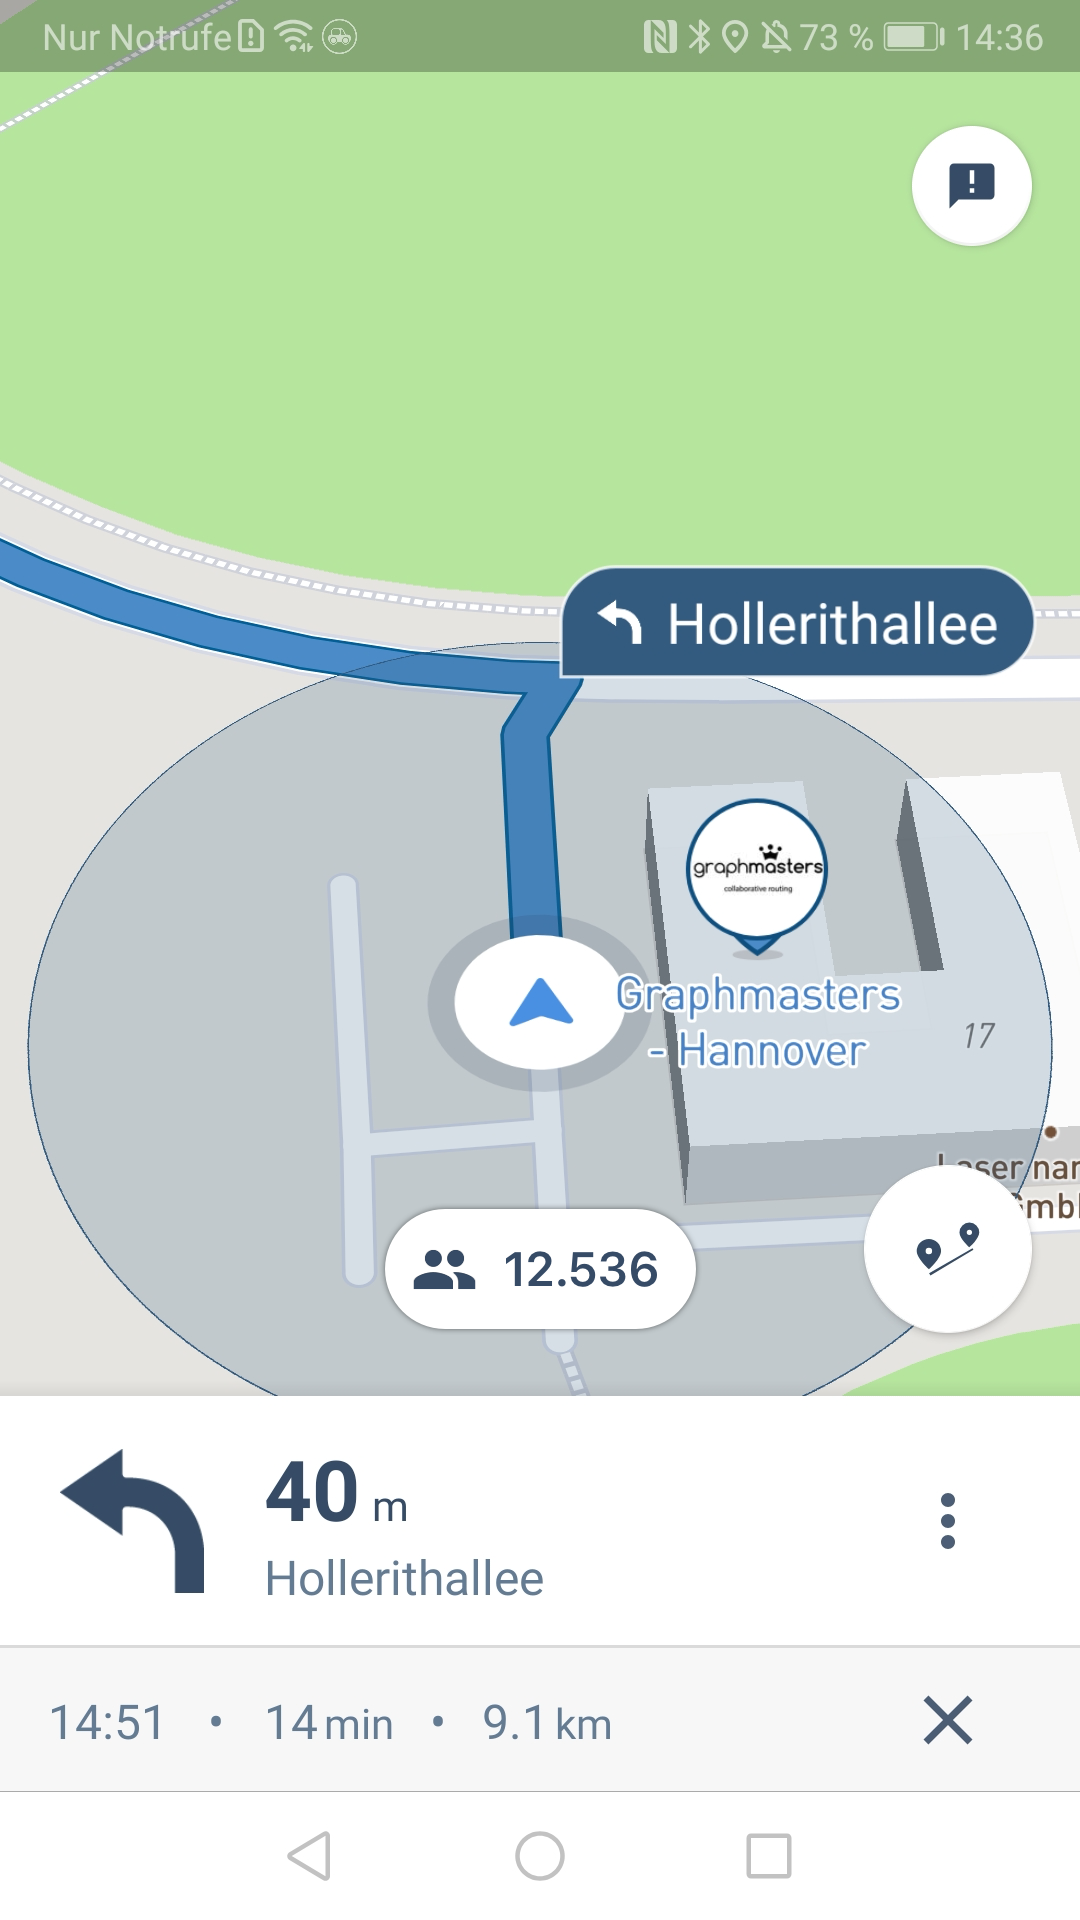
\includegraphics[width=.27\linewidth]{contents/06_model_evaluation/01_integration/res/01_collaborative_routing/prototype_1.png}
    }
    \hspace{.055\linewidth}
    \subfloat[Finales Design der Positionierung der Nutzerzahl]
    {
        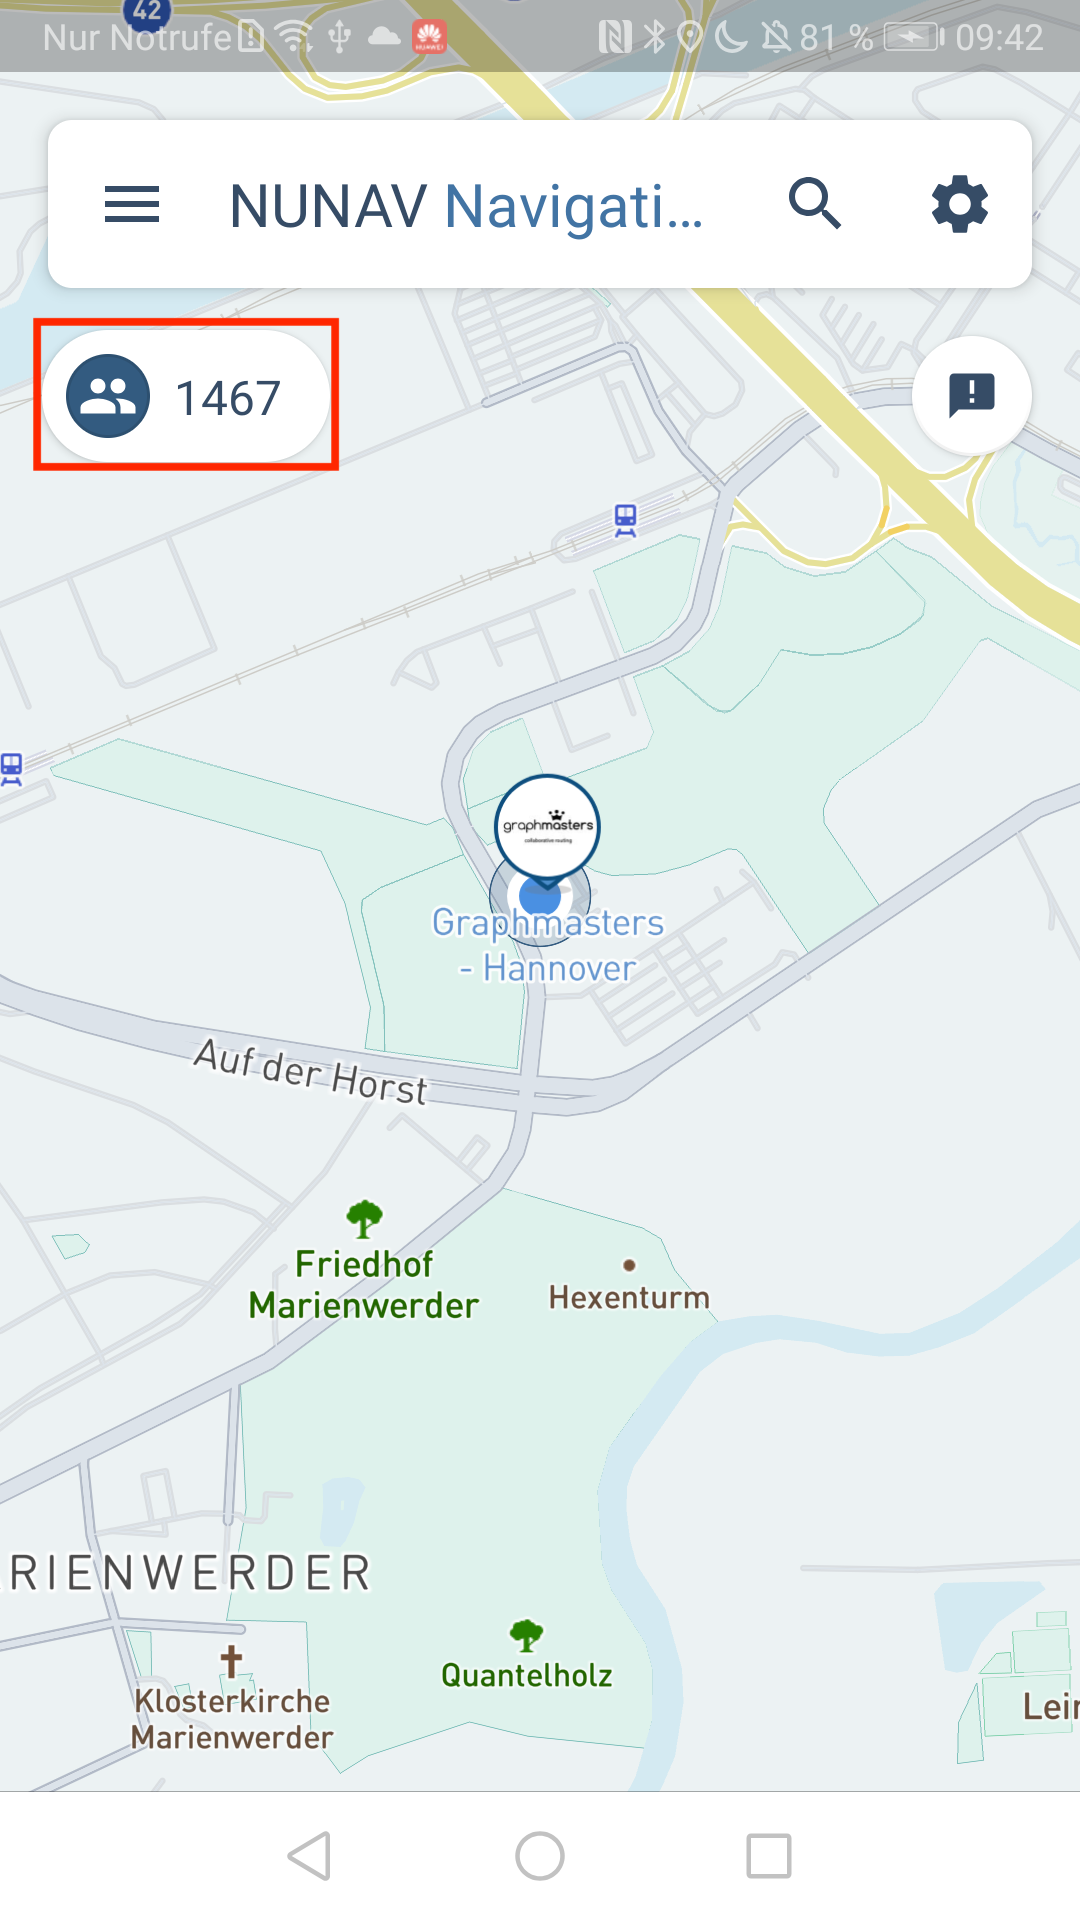
\includegraphics[width=.27\linewidth]{contents/06_model_evaluation/01_integration/res/01_collaborative_routing/final_1.png}
    }
    \hspace{.055\linewidth}
    \subfloat[Finales Design der kurzen Erklärung zum kollaborativen Routing]
    {
        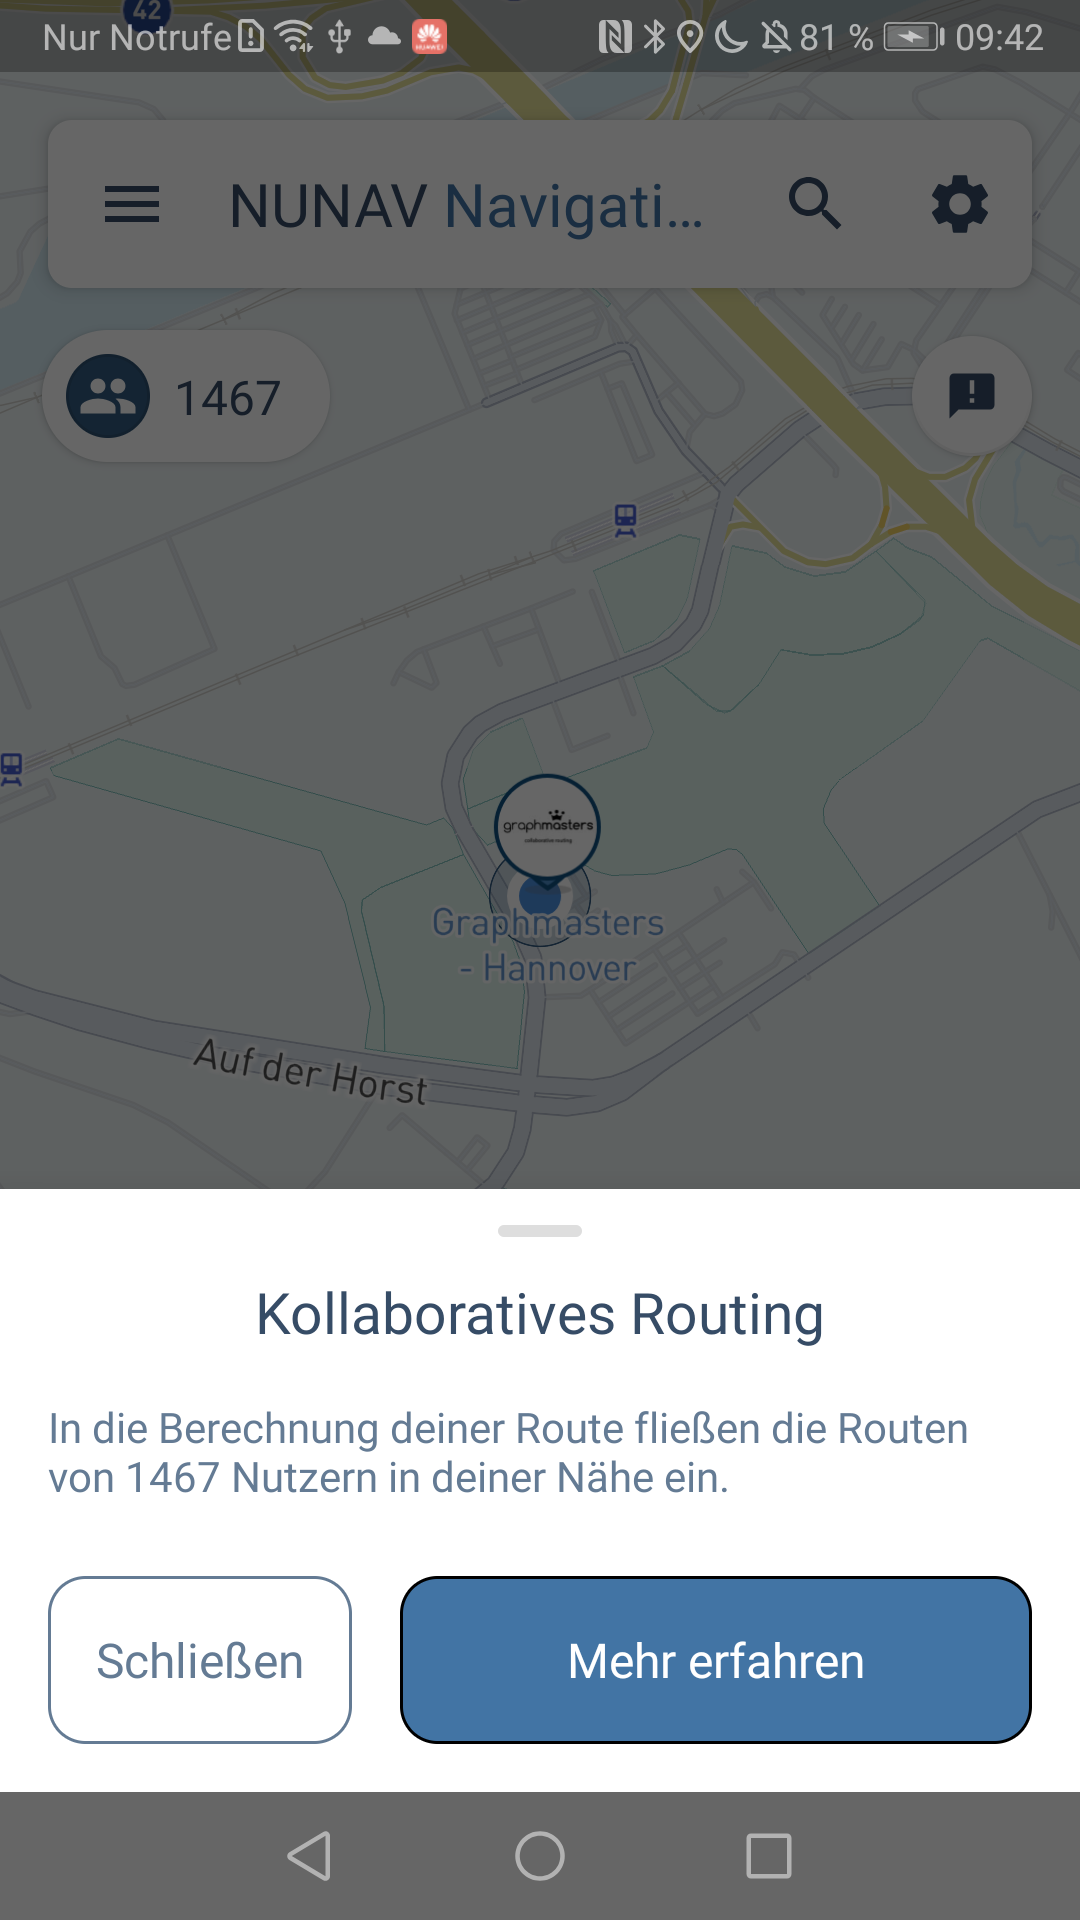
\includegraphics[width=.27\linewidth]{contents/06_model_evaluation/01_integration/res/01_collaborative_routing/final_2.png}
    }
    \caption{Prototyp und finale Designs für die Erklärung zum kollaborativem Routing}
    \label{fig:prototype_collaborative_routing}
\end{figure}

\subsubsection{Einflüsse auf die Routenberechnung}

\paragraph{[FR2]} \textit{NUNAV Navigation} muss den \textit{End Usern} die Möglichkeit bieten, abzurufen, welche Informationen zu Verkehrsereignissen (z.B. Verkehrsfluss, Sperrungen, Baustellen, Staus) in den Algorithmus einfließen.

\bigskip

Auf der Karte, welche das Hauptinteraktionselement von \textit{NUNAV Navigation} darstellt, sind Sperrungen, Baustellen und Staus bereits eingezeichnet. Wie aus dem Nutzerfeedback hervorgeht reichen diese \textit{Context}-Informationen allerdings für das Verständnis der \textit{End User} nicht aus. Daher wurde ein neuer Hilfe-Center-Artikel im Rahmen dieser Arbeit zu diesem Thema angelegt (siehe \autoref{sec:help_center_routing_data}). Dieser Artikel ist für Nutzer geeignet, welche NUNAV zum ersten Mal wie Ayla oder noch nicht lange wie Michael verwenden. So können sie sich anhand der Daten auf der Karte im Anschluss an das Lesen des Artikels die verschiedenen Routen besser erklären.

Dieser Beitrag wurde ebenfalls vor dem Start der Navigation erreichbar gemacht. Um die Standardkartenansicht nicht durch mehrere Möglichkeiten zum Aufrufen von Hilfe-Center-Artikeln zu überladen, wurde die Möglichkeit, zu dieser Erklörung zu gelangen, in die Routen-Vorschau integriert. Auch für diese wurden mehrere Prototypen erstellt, wobei bei der finalen Entscheidung darauf geachtet wurde, dass die Aufrufmöglichkeit nicht zu viel Platz einnimmt und der Text neugierig macht. Die verschiedenen Prototypen sind in \autoref{fig:prototype_routing_explanation} zu sehen.

\begin{figure}[htb!]
    \centering
    \subfloat[1. Prototyp zur Positionierung des Aufrufs der Erklärung]
    {
        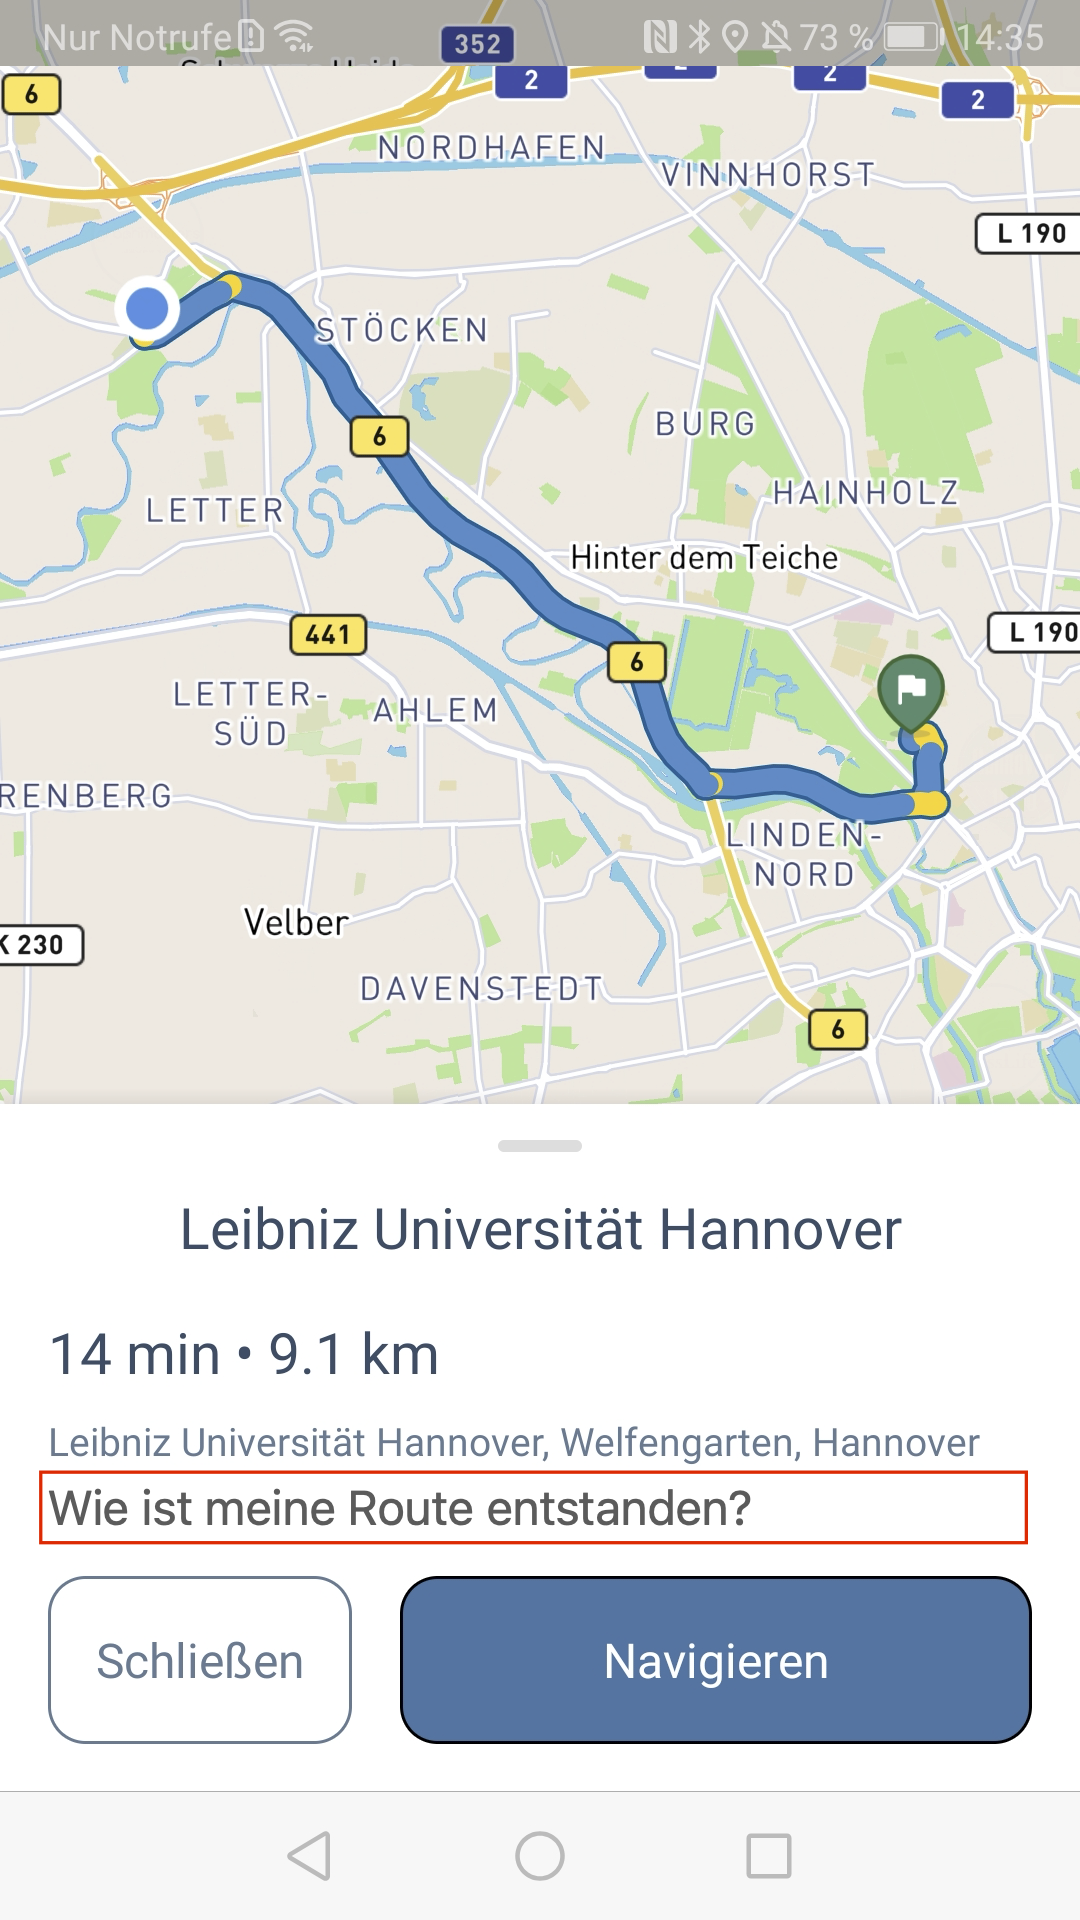
\includegraphics[width=.27\textwidth]{contents/06_model_evaluation/01_integration/res/02_routing_algorithm/prototype_1.png}
    }
    \hspace{.055\textwidth}
    \subfloat[Alternativer Prototyp zur Positionierung des Aufrufs der Erklärung]
    {
        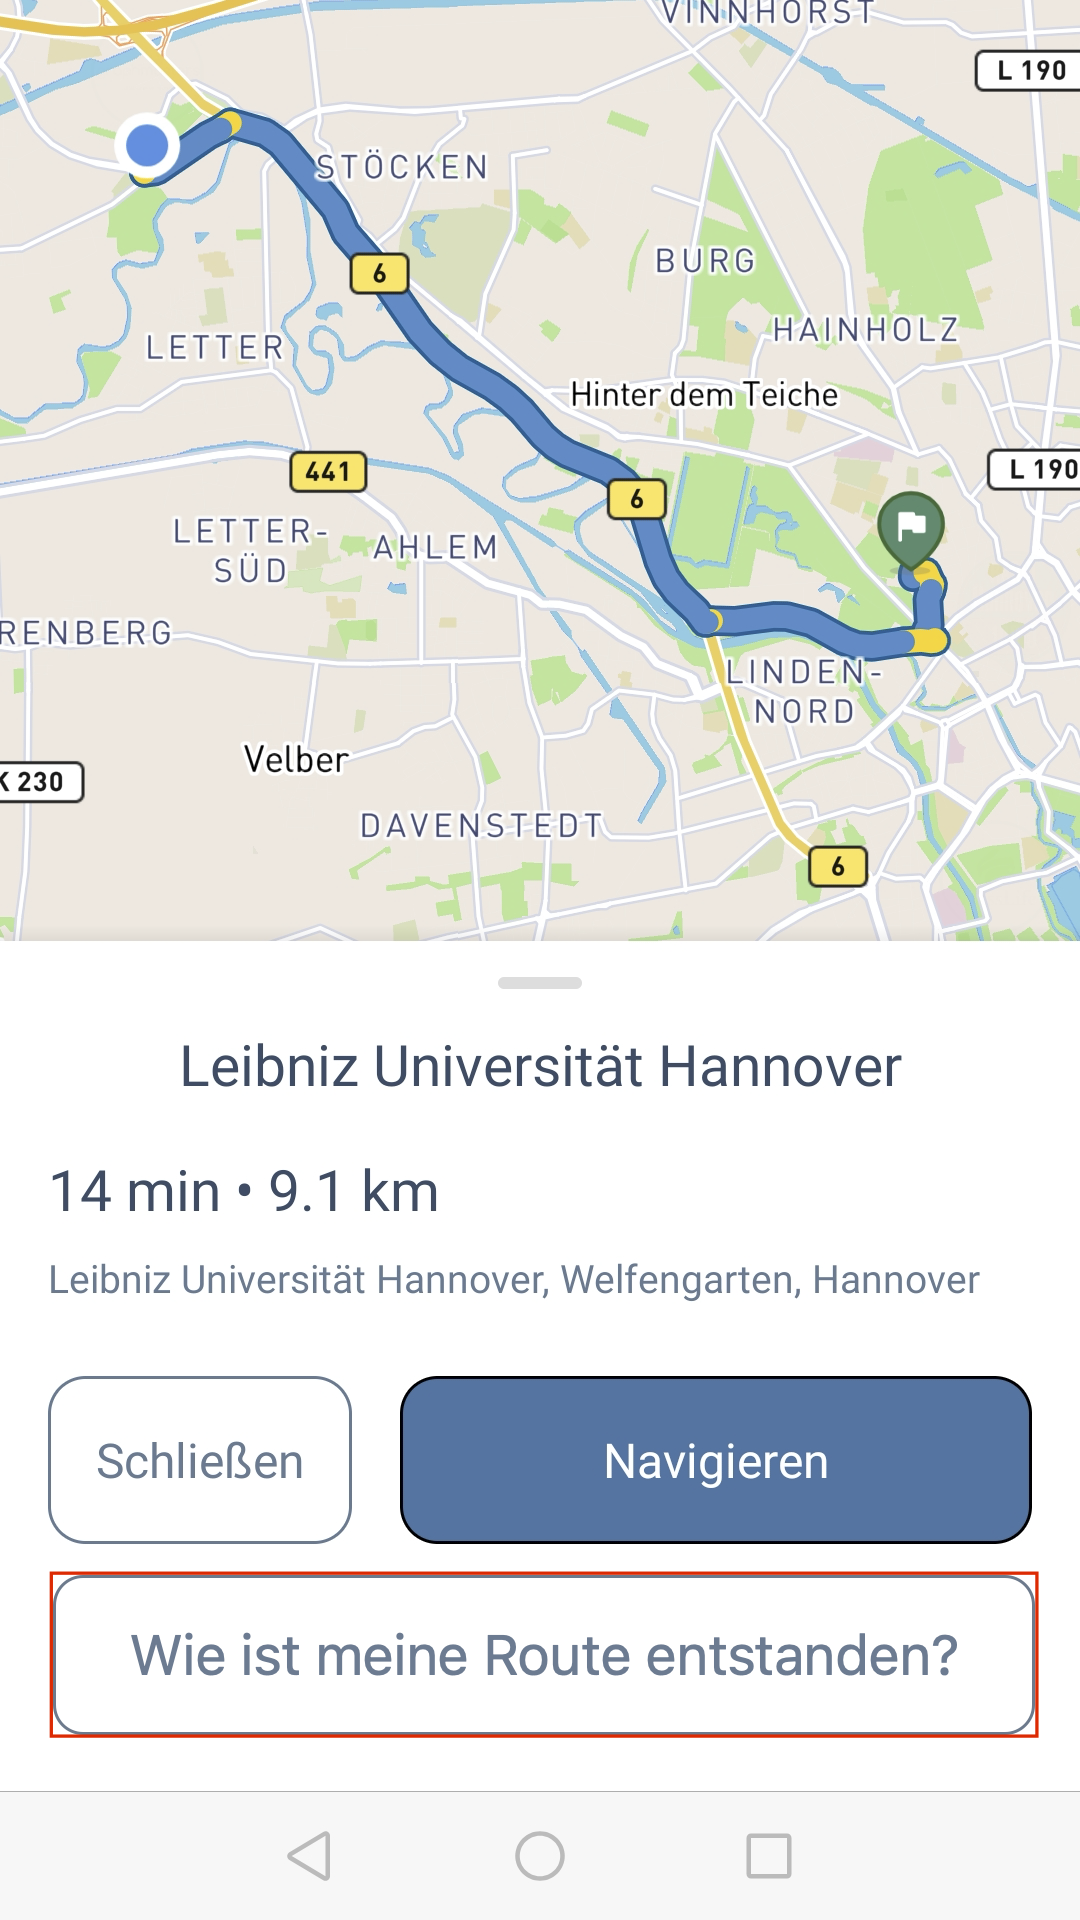
\includegraphics[width=.27\textwidth]{contents/06_model_evaluation/01_integration/res/02_routing_algorithm/prototype_2.png}
    }
    \hspace{.055\textwidth}
    \subfloat[Finales Design zur Positionierung des Aufrufs der Erklärung]
    {
        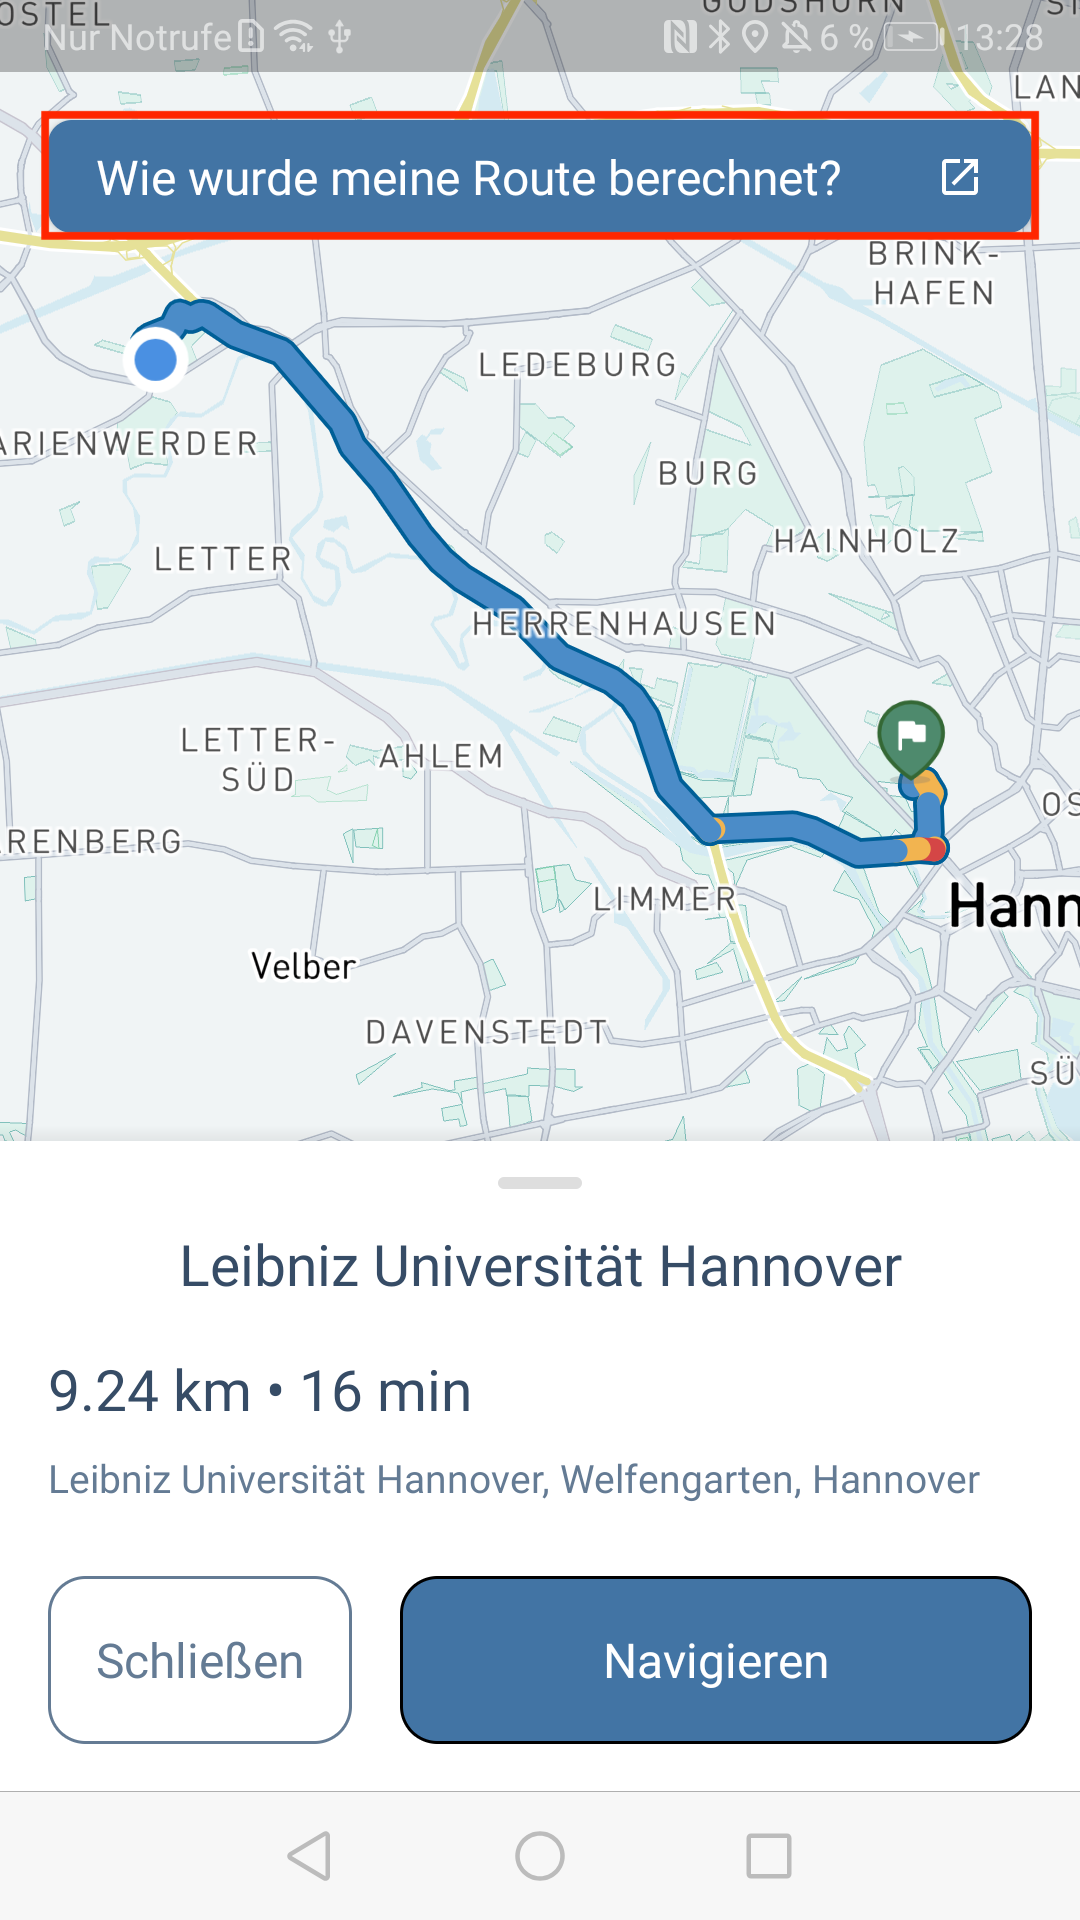
\includegraphics[width=.27\textwidth]{contents/06_model_evaluation/01_integration/res/02_routing_algorithm/final_1.png}
    }
    \caption{Prototyp und finale Designs für den Aufruf der Erklärung zu Einflüssen auf die Routenberechnung}
    \label{fig:prototype_routing_explanation}
\end{figure}

\subsubsection{Verkehrsaufkommen}
\label{sec:traffic_volume_definition}

\paragraph{[FR3]} \textit{NUNAV Navigation} muss den \textit{End Usern} während der Navigation Informationen zum Verkehrsgeschehen auf der aktuellen Route liefern.

Wie aus der Persona von Michael hervorgeht, wundert er sich zum Teil, warum \textit{NUNAV Navigation} aus seiner Sicht \glqq komische\grqq{} Routen vorschlägt. Ein Erklärungsansatz ist, das Verkehrsgeschehen auf der aktuellen Route anzuzeigen. Diese \textit{Context}-Information soll dabei helfen zu verstehen, warum \textit{NUNAV Navigation} andere Routen wählt. 

Dies ist allerdings nicht trivial, da die Berechnung des Verkehrsaufkommens und dessen subjektive Wahrnehmung der \textit{End User} nicht klar ist. Ein weiteres Problem ist, dass es nicht möglich ist, zu berechnen, welche Route für Nutzer auf der gleichen Strecke subjektiv als \glqq normal\grqq{} empfunden wird. Nachdem mehrere Lösungsansätze für dieses Problem in kleinen Runden bei \textit{Graphmasters} diskutiert wurden, wird als Lösung die Berechnung des Verhältnisses von durchschnittlicher Dauer der Route zu aktueller Dauer als Basiswert genommen. Die Daten werden dabei durch \textit{Nugraph} zur Verfügung gestellt und im Rahmen dieser Arbeit im \textit{BFF} auf die Stufen \glqq wenig Verkehr\grqq{}, \glqq mäßiger Verkehr\grqq{} und \glqq viel Verkehr\grqq{} abgebildet. Außerdem gibt es eine \glqq normale\grqq{} Verkehrssituation, in der den \textit{End Usern} keine Erklärung angezeigt wird. Die Abbildungsfunktion ist in den Zusatzmaterialien zu finden. Die Schwellwerte wurden intern durch Testfahrten ermittelt.

Die Informationen können \textit{End User} auf drei Wegen erhalten. Zunächst werden die Informationen in der Routenvorschau angezeigt. Dabei wird die Gesamtfahrzeit für die Route je nach Verkehrsaufkommen grün (wenig Verkehr), Standardtextfarbe (normaler Verkehr), orange (mäßiger Verkehr) und rot (viel Verkehr) dargestellt. Da im ersten Prototypen aufgefallen ist, dass die Farben alleine nicht aussagekräftig sind (siehe \autoref{fig:prototype_traffic_volume_route}, (a)), wurde zusätzlich ein kurzer Erklärungstext eingefügt (siehe \autoref{fig:prototype_traffic_volume_route}, (b)). Dieser ist bei \glqq normalem\grqq{} nicht zu sehen. So lernen die \textit{End User} mit der Zeit die Bedeutung der Farben. Eine Übersicht mit allen Prototypen ist in \autoref{sec:appendix_traffic_volume} zu finden.

Außerdem werden während der gesamten Navigation die Ankunftszeit und die Fahrzeit in der entsprechenden Farbe angezeigt und bei sich ändernder Verkehrssituation auch aktualisiert.

\begin{figure}[htb!]
    \centering
    \subfloat[Prototyp zur Darstellung des aktuellen Verkehrsaufkommens in der Routenvorschau]
    {
        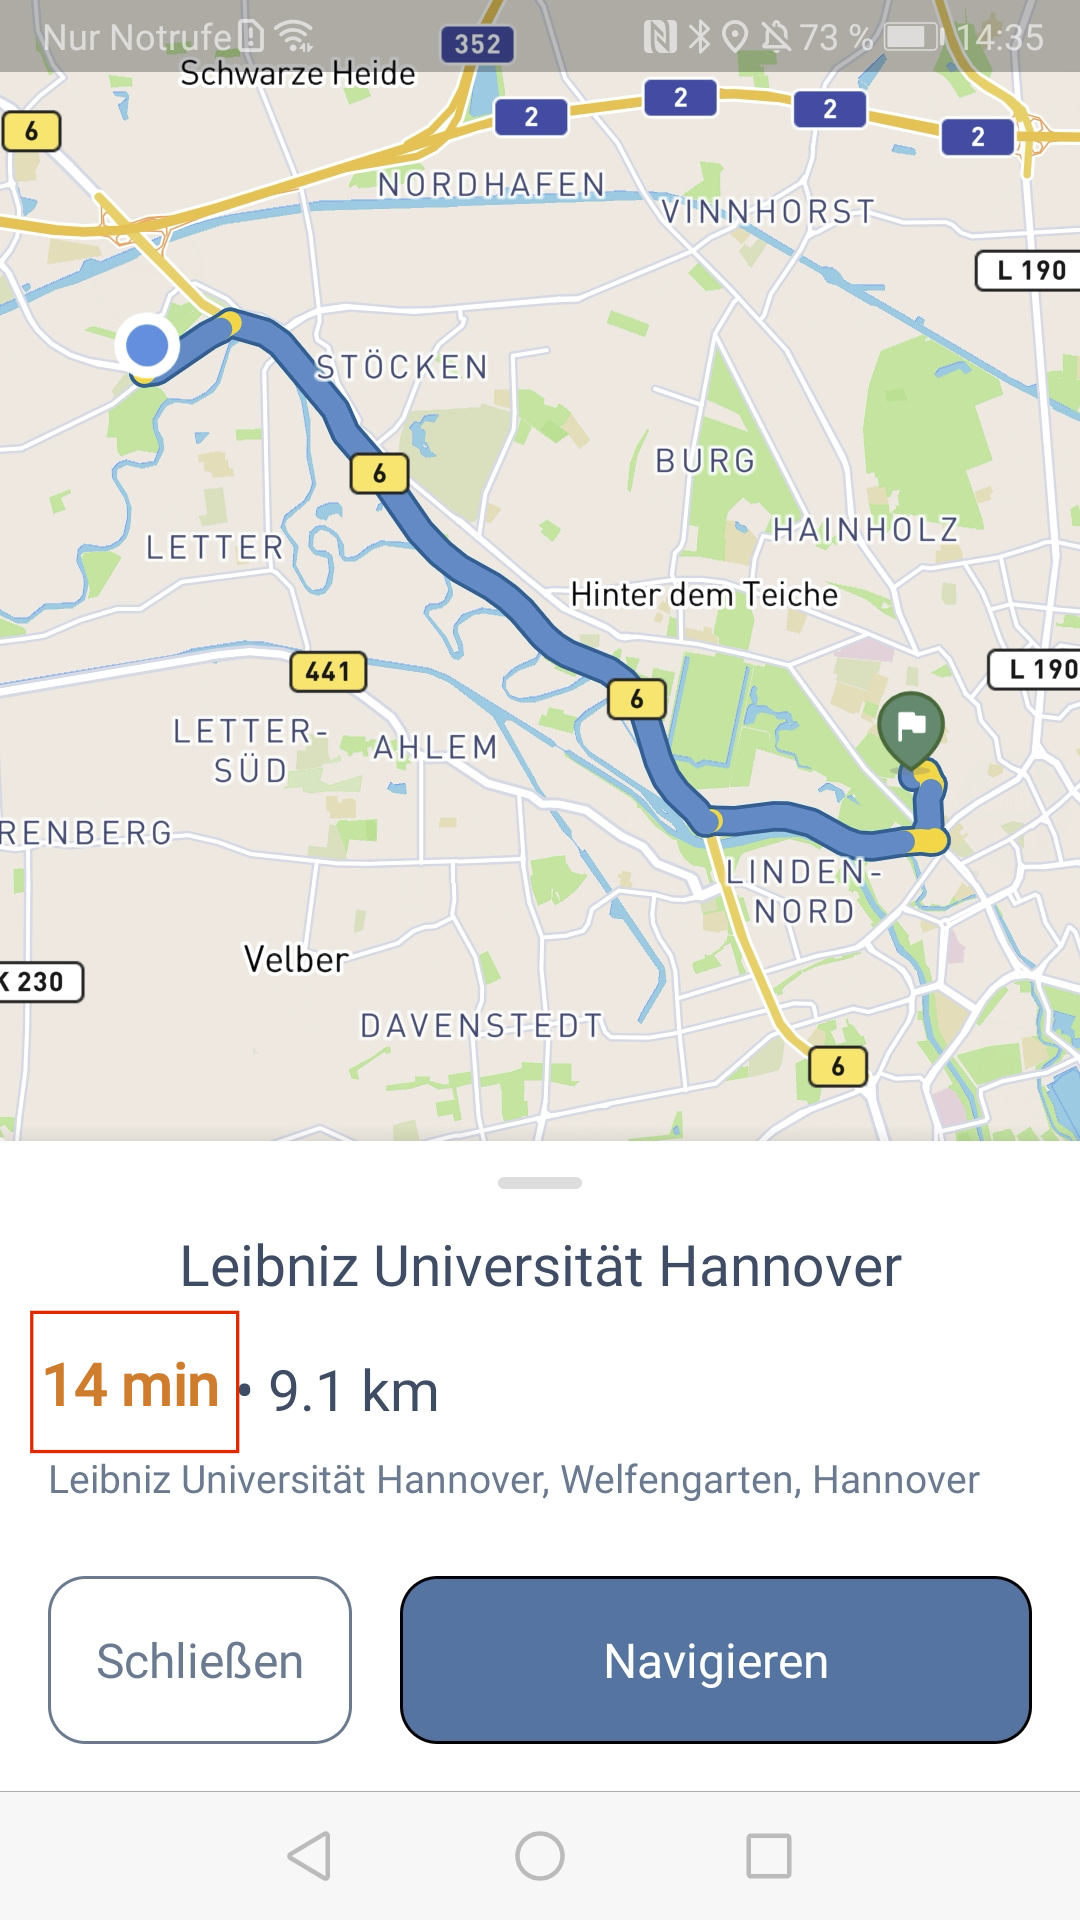
\includegraphics[width=.27\textwidth]{contents/06_model_evaluation/01_integration/res/03_traffic_volume/prototype_11.png}
    }
    \hspace{.055\textwidth}
    \subfloat[Finales Design zur Darstellung des aktuellen Verkehrsaufkommens in der Routenvorschau]
    {
        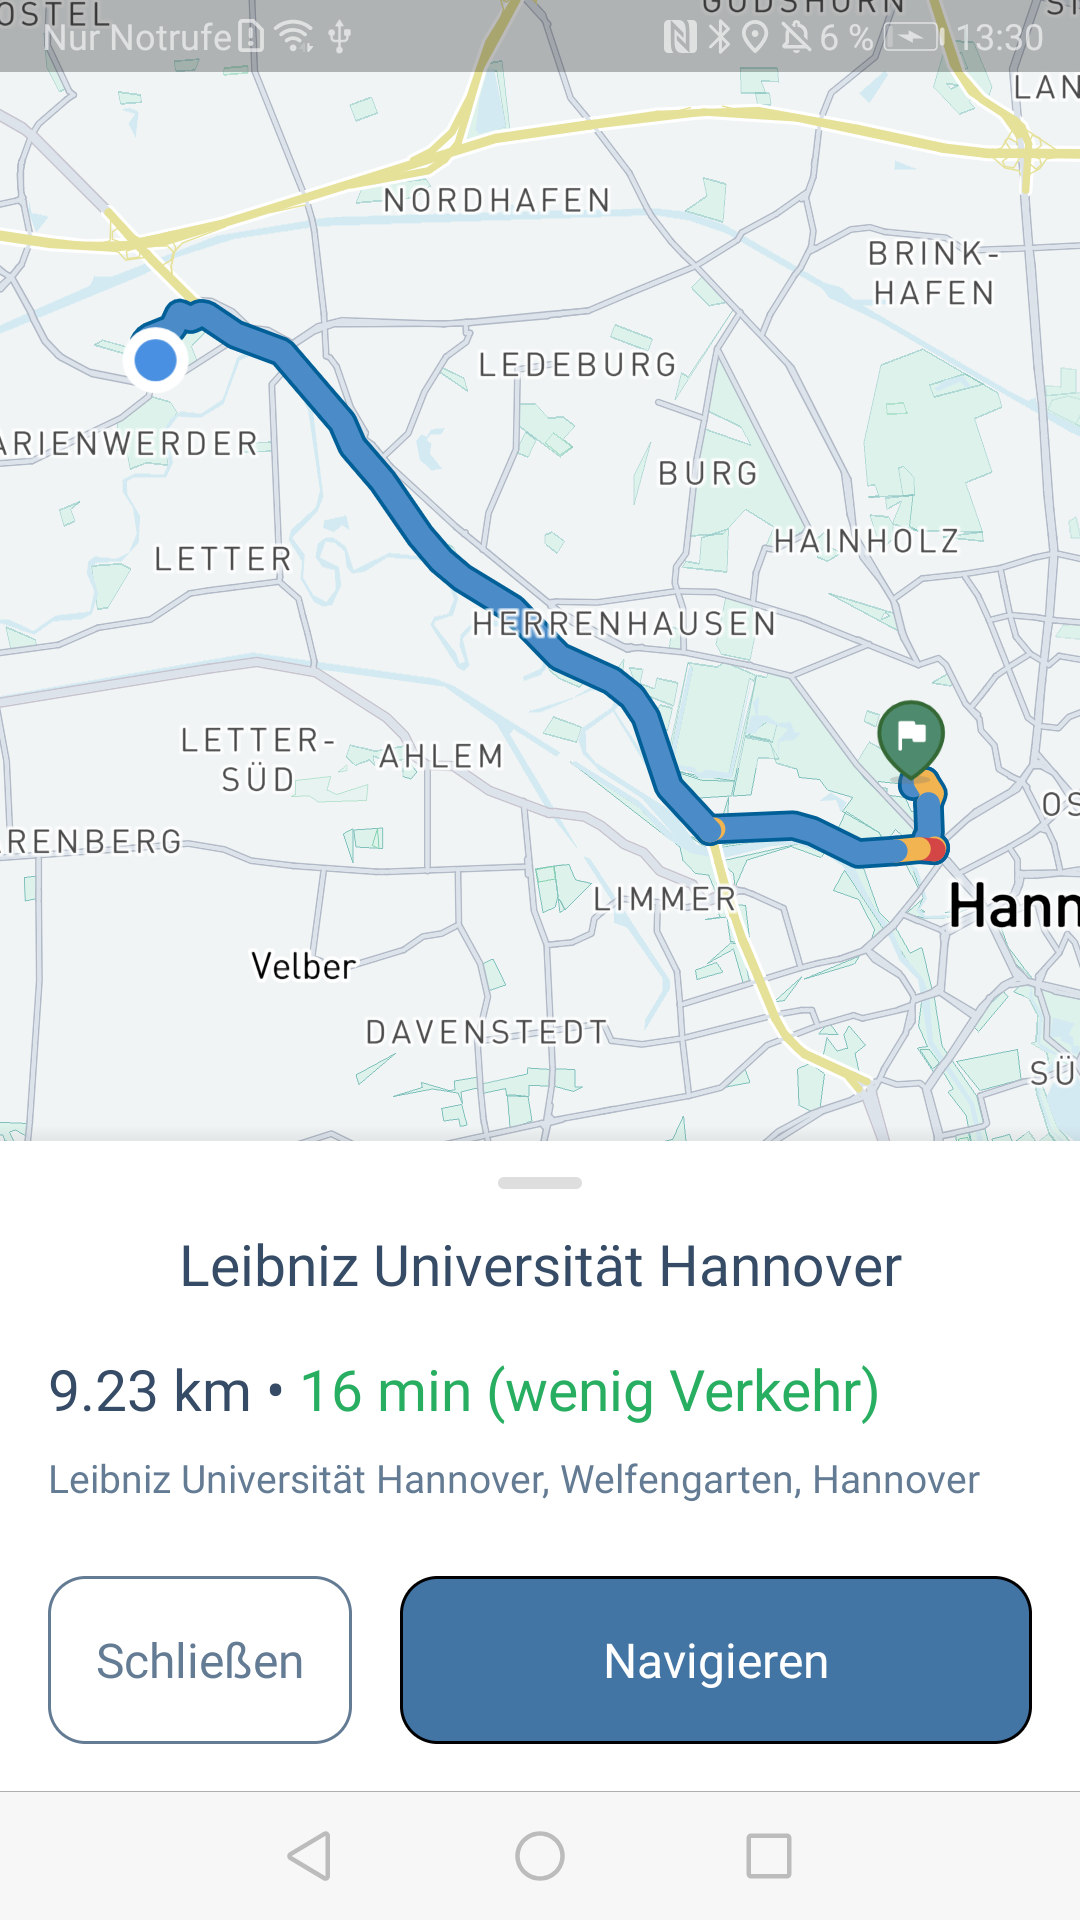
\includegraphics[width=.27\textwidth]{contents/06_model_evaluation/01_integration/res/03_traffic_volume/final_10.png}
    }
    \hspace{.055\textwidth}
    \subfloat[Finales Design zur Darstellung des aktuellen Verkehrsaufkommens während der Navigation]
    {
        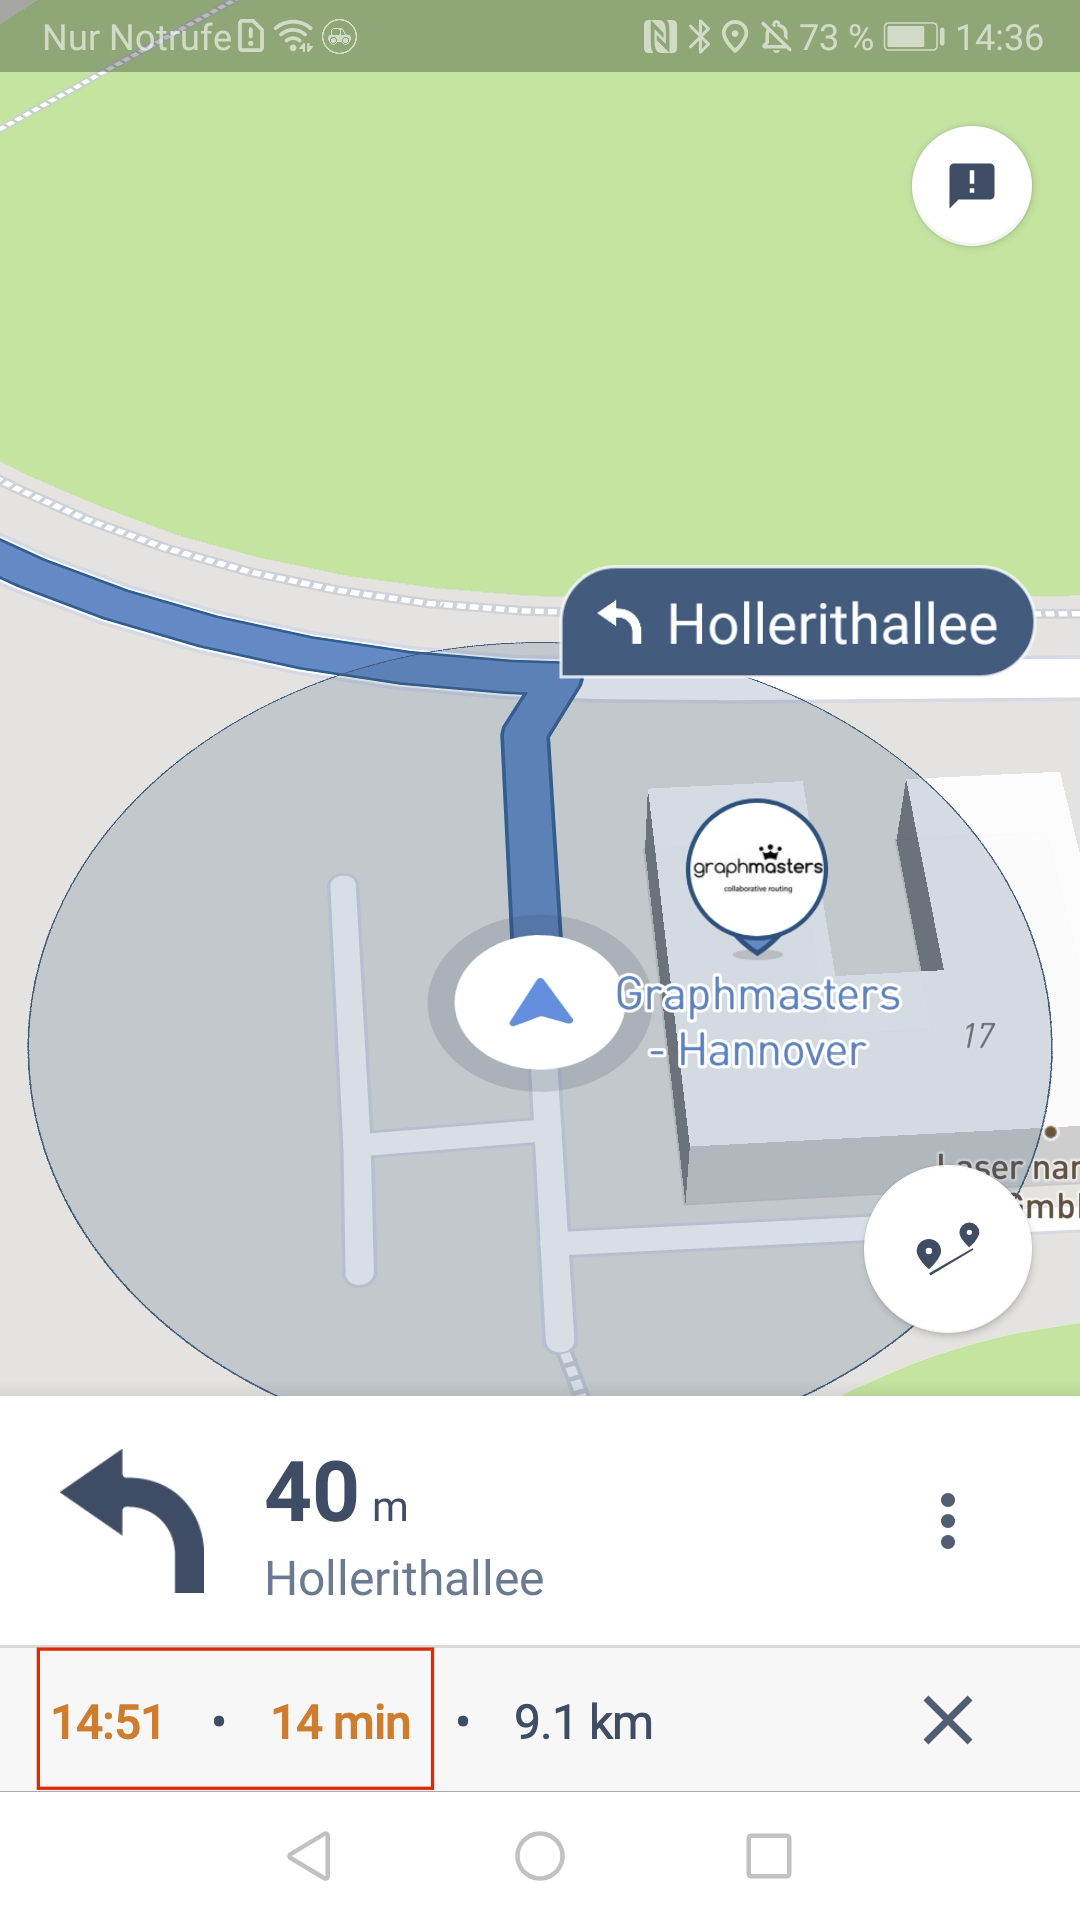
\includegraphics[width=.27\textwidth]{contents/06_model_evaluation/01_integration/res/03_traffic_volume/final_20.png}
    }
    \caption{Prototyp und finale Designs für die Erklärung zum kollaborativem Routing}
    \label{fig:prototype_traffic_volume_route}
\end{figure}

Des Weiteren ist das Sprachkommando, welches bei Start der Navigation gegeben wird, je nach Verkehrssituation unterschiedlich (siehe \autoref{tab:voice_commands_traffic_volume}).

\begin{table}[bht!]
    \begin{tabular}{p{.25\textwidth}p{.71\textwidth}}
        \hline
        Verkehrsaufkommen        & Sprachkommando \\
        \toprule
        wenig & Heute sind die Straßen frei. Du wirst dein Ziel <Zielname> um <Uhrzeit> erreichen. \\
        \tablerowspacing
        normal & Du wirst dein Ziel <Zielname> um <Uhrzeit> erreichen. \\
        \tablerowspacing
        mäßig & Da heute etwas mehr los ist, wirst du dein Ziel <Zielname> um <Uhrzeit> erreichen. \\
        \tablerowspacing
        viel & Da heute sehr viel los ist, wirst du dein Ziel <Zielname> um <Uhrzeit> erreichen. \\
        \toprule
    \end{tabular}
\caption{Sprachkommandos zum Start der Navigation abhängig von der Verkehrssituation}
\label{tab:voice_commands_traffic_volume}
\end{table}

\subsubsection{GPS-Qualität}
\label{sec:gps_accuracy_definition}

\paragraph{[FR4]} Wenn die Genauigkeit der Positionierung unzuverlässig ist, muss \textit{NUNAV Navigation} den \textit{End Usern} anzeigen, dass die Positionierung aktuell nicht zuverlässig ist.

Die letzte entwickelte Erklärung betrifft den Aspekt der \textit{Scrutability}. Ziel ist es \textit{End Usern} anzuzeigen, wenn sie sich aktuell auf die Position auf der Route nicht verlassen können. Dies ist zum Beispiel in Tunneln der Fall und besonders kritisch, wenn in Kürze ein Abbiege-Kommando erfolgt und somit an der falschen Stelle kommt. Bewusst wurde auf die technische Bezeichnung \glqq GPS\grqq{} verzichtet.

\begin{figure}[htb!]
    \centering
    \subfloat[Prototyp zum Design bei schlechtem GPS]
    {
        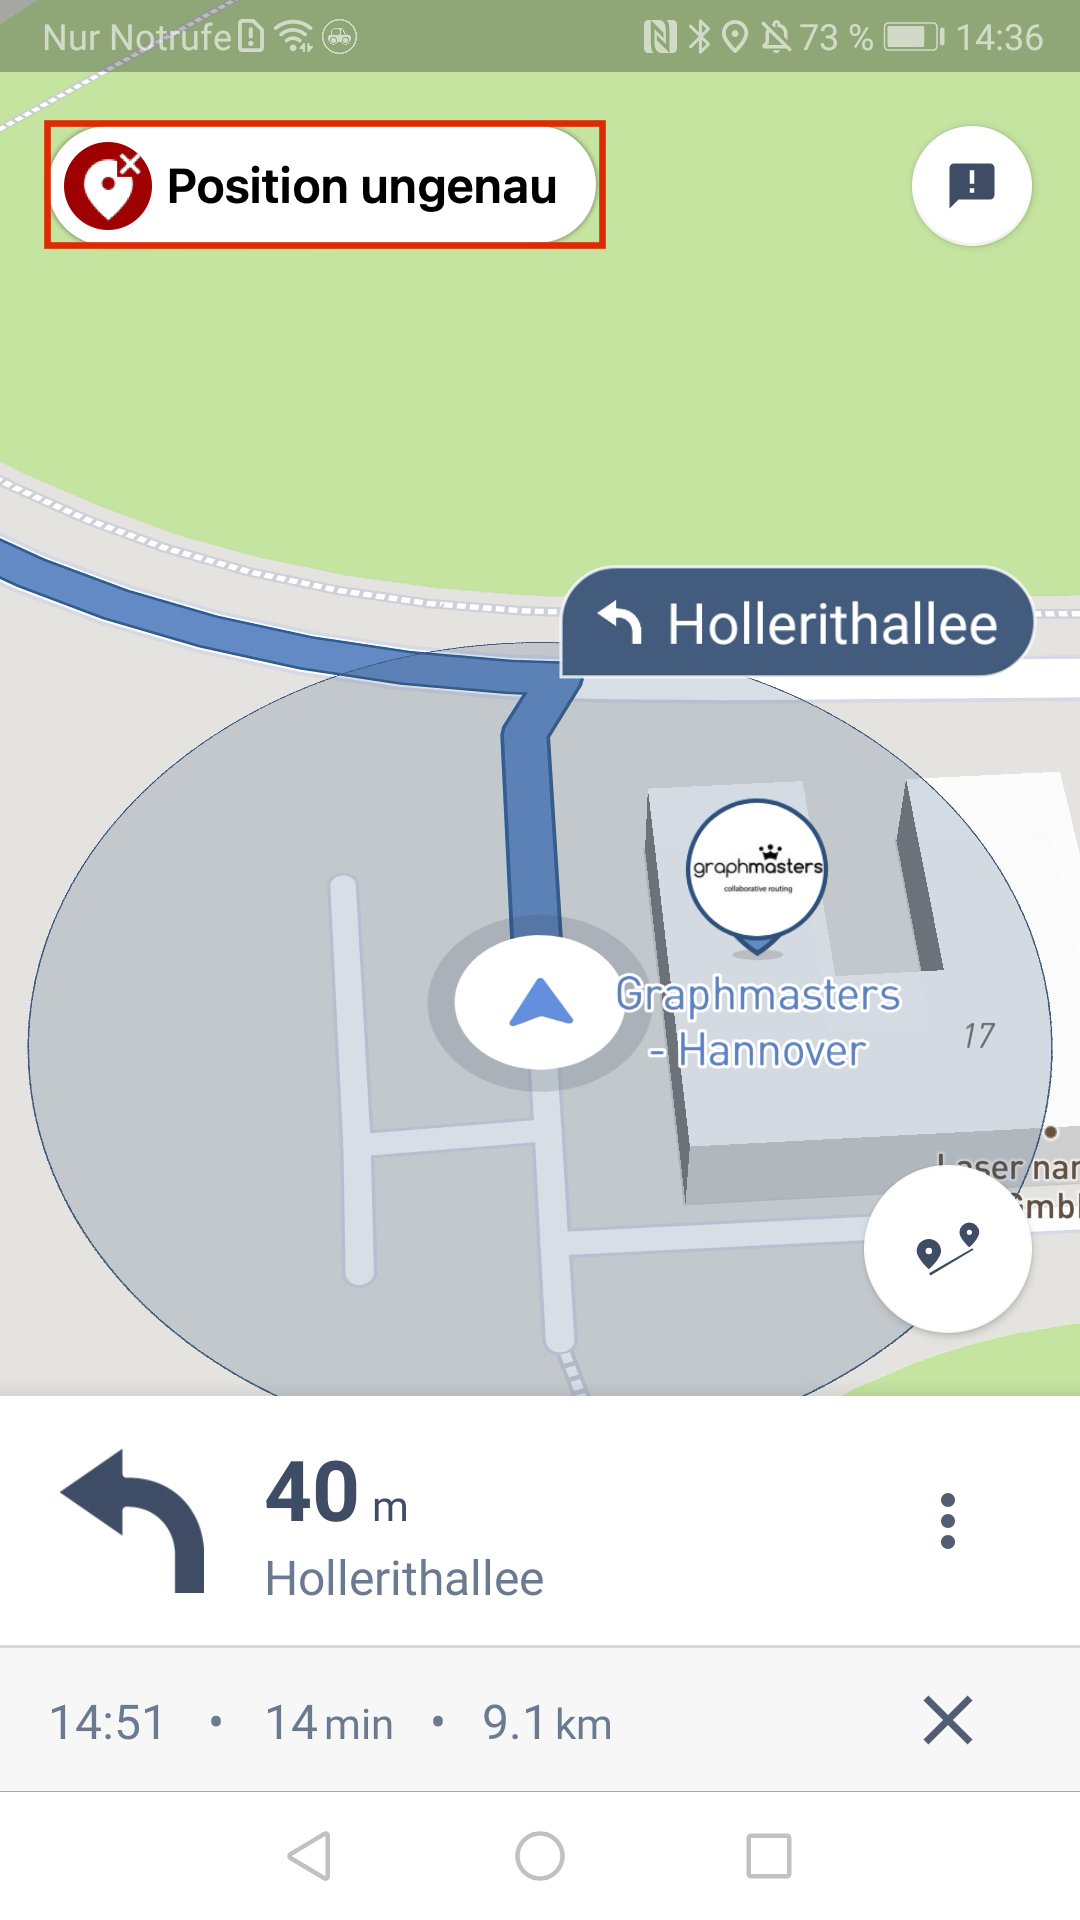
\includegraphics[width=.27\textwidth]{contents/06_model_evaluation/01_integration/res/04_position_accuracy/prototype_1.png}
    }
    \hspace{.055\textwidth}
    \subfloat[Finales Design bei schlechtem GPS]
    {
        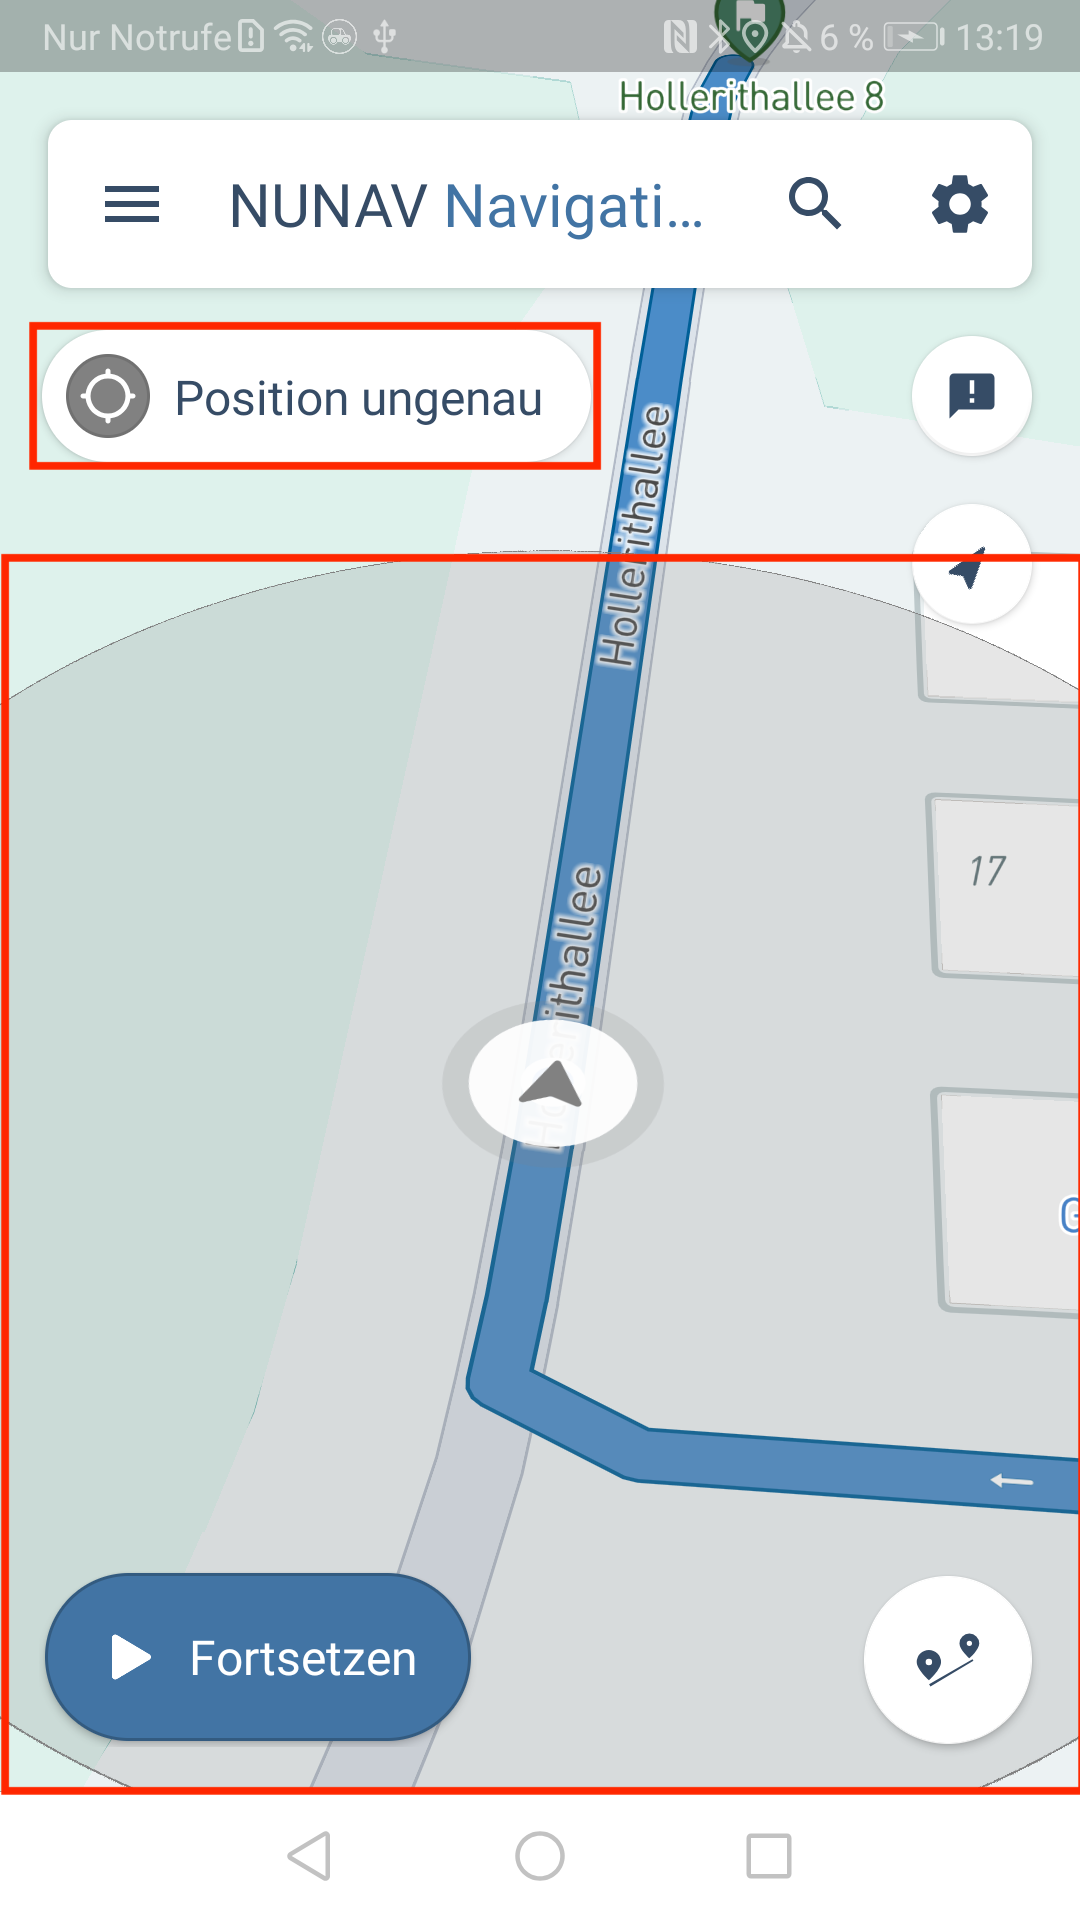
\includegraphics[width=.27\textwidth]{contents/06_model_evaluation/01_integration/res/04_position_accuracy/final_1.png}
    }
    \caption{Prototyp und finales Design für die Anzeige von schlechtem GPS während der Navigation}
    \label{fig:prototype_position_accuracy}
\end{figure}

Für die Entscheidung, wann das GPS ungenau ist, wurde innerhalb der \textit{NUNAV Navigation}-App ein neuer Algorithmus integriert, der diese trifft. Dabei spielt nicht nur die Genauigkeit, welche durch das GPS-Modul des Gerätes ermittelt wird, eine Rolle, sondern auch die Zeit, wann das letzte GPS-Update kam, da bei sehr schlechtem GPS keine Positionsupdates mehr vom Gerät geliefert werden. Der Algorithmus ist in den Zusatzmaterialien zu finden.

Als Design wurde im ersten Entwurf lediglich ein \textit{Growl} angezeigt und die Sprachansage \glqq Position ungenau\grqq{} ausgegeben. Insbesondere, wenn zum gleichen Zeitpunkt weitere \textit{Growls} angezeigt werden und die Sprachansagen vom \textit{End User} generell deaktiviert sind, hat sich die Sichtbarkeit bei Testfahrten als ungenügend herausgestellt. Daher wurde im finalen Entwurf zusätzlich das Positions-Icon auf der Karte und der Kreis, welcher die Genauigkeit der Position anzeigt, ausgegraut (siehe \autoref{fig:prototype_position_accuracy}, (b)).

\subsection{Umsetzung}

